% Chapter 4: Data, Readiness and Design Evaluation
\chapter{Data, Readiness and Design Evaluation}\label{chap:4}
\label{ch:data}

After a design has been created (Chapter~\ref{chap:3}), the work moves to the pages of the groups \ui{Design} and
\ui{Project} in the navigation tree. The \ui{Data} page holds the design matrix and the measured responses;
\ui{Data Readiness} checks whether the data are good enough for modeling and optimization and suggests extra runs;
\ui{Design Evaluation} judges the design itself, before or after the experiment, without using any response values.
The project pages \ui{Summary}, \ui{Notes} and \ui{Column Graphs}, the \ui{Coefficient Table} and the tool
\ui{Data Normalization} complete the picture. The examples use the built-in case studies (\menupath{File
$\rightarrow$ Case Studies\dots}).

\section{The Data page}
\label{sec:ch04-data}

\paragraph{Purpose.} The \ui{Data} page (title ``Data \& Design'') shows every run of the design with its factor
settings and is the place where the measured responses are entered.

\begin{figure}[htbp]
\centering
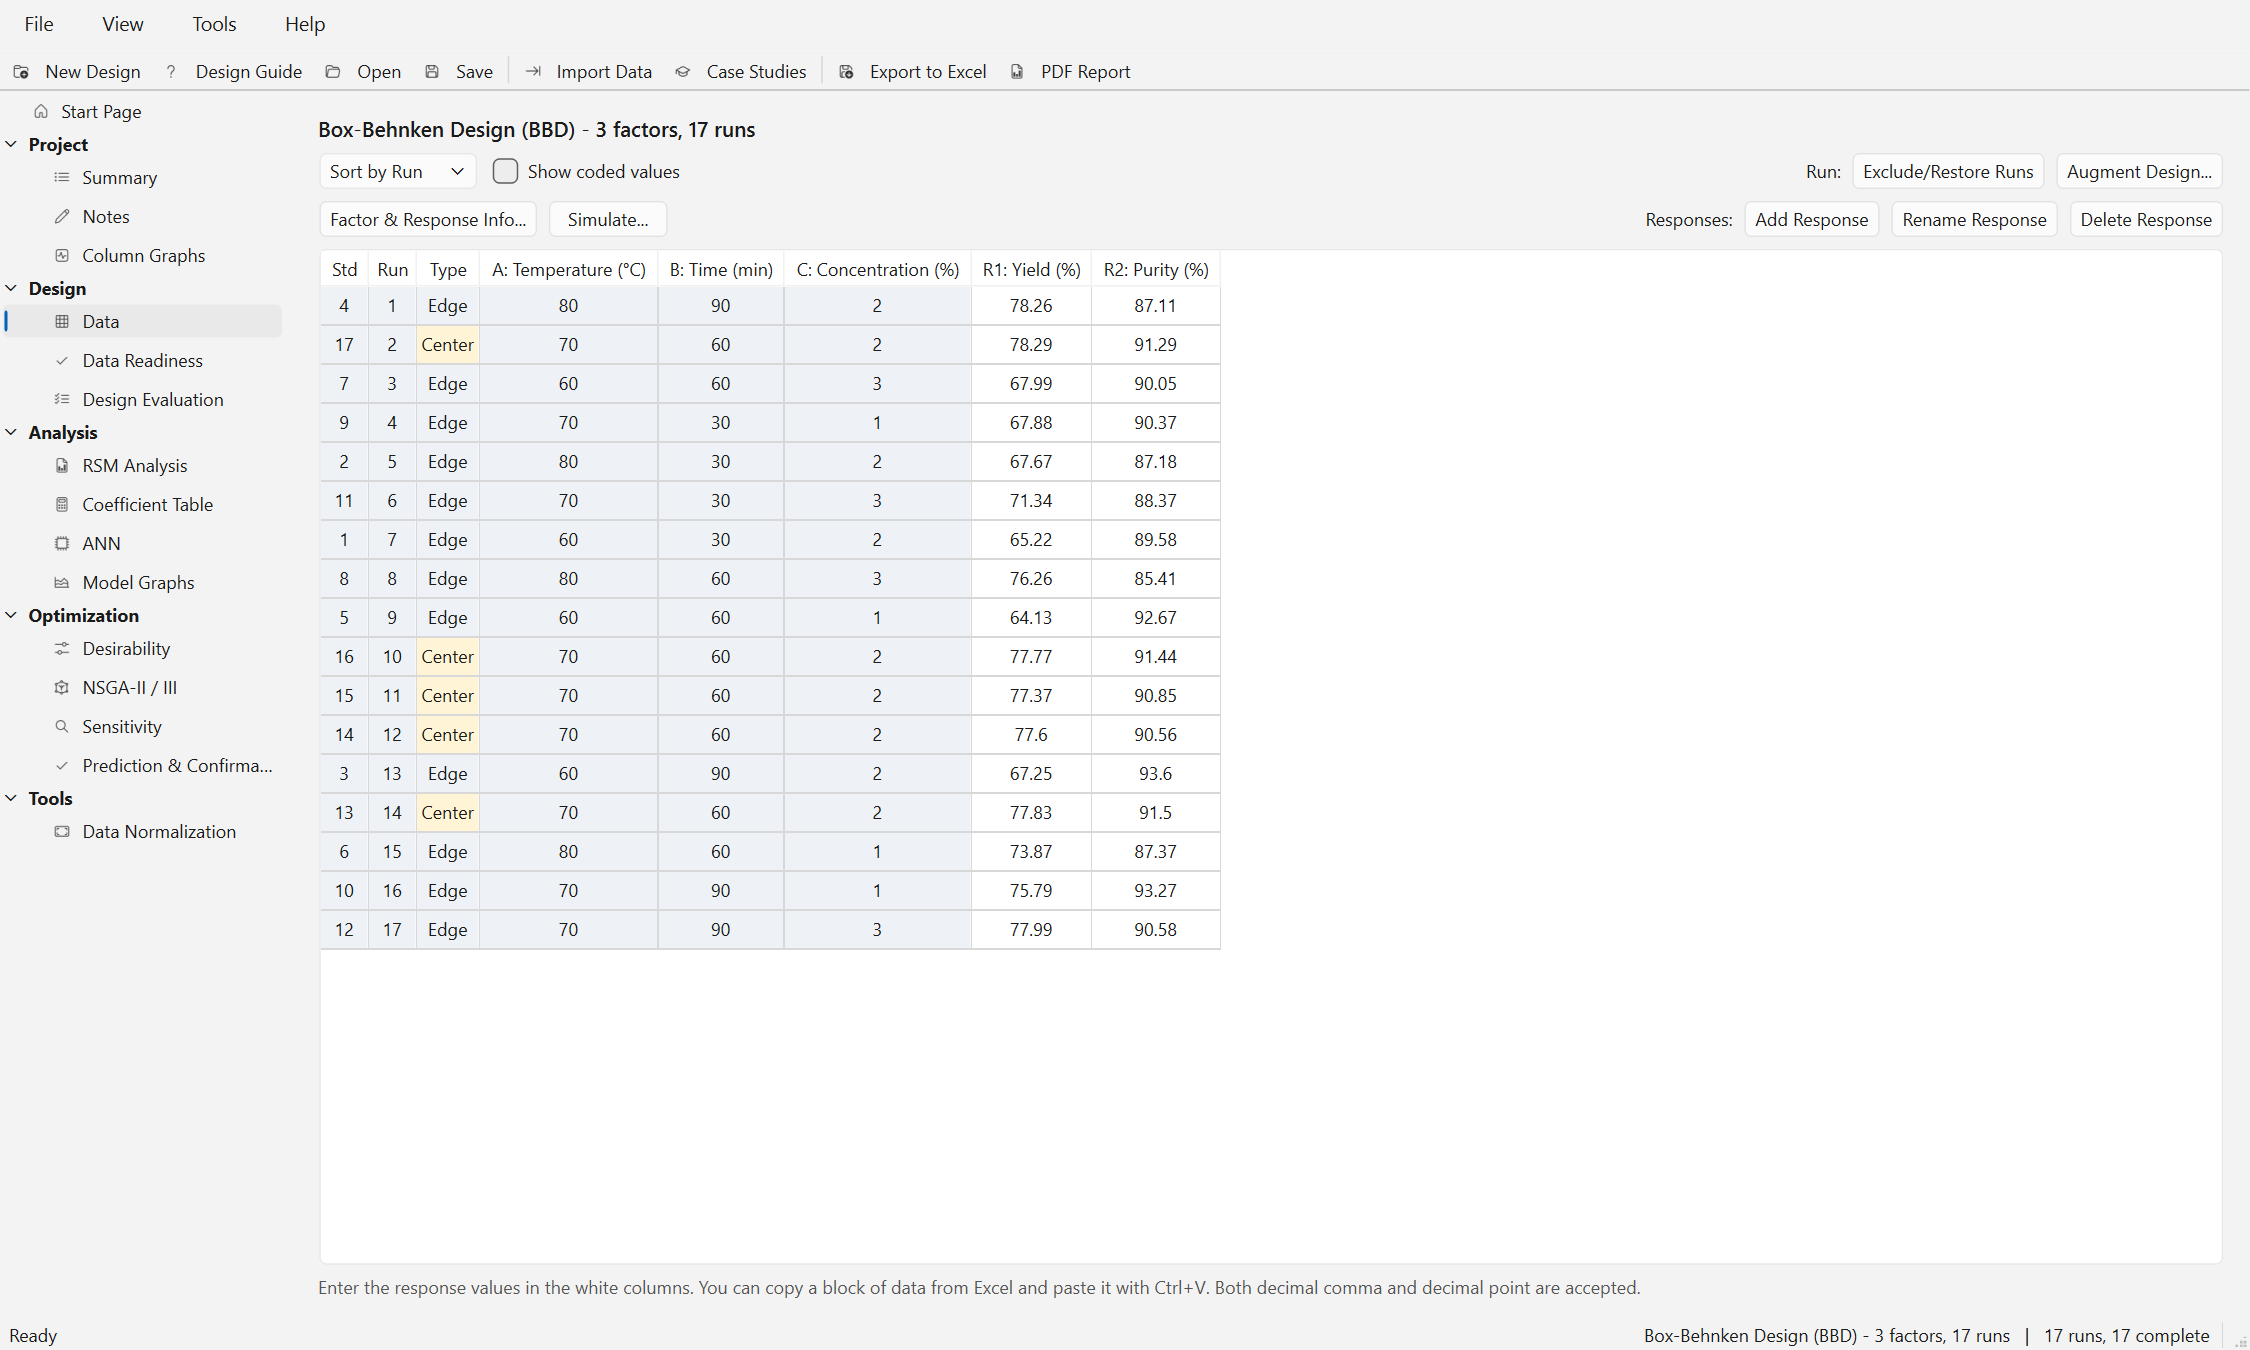
\includegraphics[width=\linewidth]{data_page.png}
\caption{Data page of the case study ``Extraction Optimization (Box-Behnken)'': 17 runs sorted by run order, point
types Edge and Center, grey read-only factor columns and white response columns Yield and Purity.}
\label{fig:ch04-datapage}
\end{figure}

\paragraph{Layout.} The bold line at the top is the design description, for example ``Box-Behnken Design (BBD) - 3
factors, 17 runs''. The first toolbar row contains the sort selector (\ui{Sort by Run} or \ui{Sort by Std}), the
check box \ui{Show coded values} (\ui{Show pseudo-components} for mixtures), \ui{Add Rows} and \ui{Delete Selected
Rows} (historical data only), \ui{Exclude/Restore Runs} and \ui{Augment Design\dots} (not for historical data).
The second row contains \ui{Factor \& Response Info\dots}, \ui{Simulate\dots} and the response buttons \ui{Add
Response}, \ui{Rename Response} and \ui{Delete Response}. The status bar at the bottom of the window repeats the
design description and shows ``N runs, F complete'' (F = runs with all responses filled) and, if any, ``m
excluded''.

\paragraph{Columns.} Table~\ref{tab:ch04-columns} describes the columns of the data sheet.

\begin{table}[htbp]
\centering
\caption{Columns of the data sheet.}
\label{tab:ch04-columns}
\small
\begin{tabularx}{\linewidth}{@{}p{3.2cm}X@{}}
\toprule
Column & Meaning \\
\midrule
\ui{Std} & Standard order: the position of the run in the design as constructed (1, 2, \dots). \\
\ui{Run} & Run order: the randomized order in which the experiments must be performed. \\
\ui{Block} & Block number (only when the design has more than one block). \\
\ui{WP} & Whole plot (split-plot designs only). \\
\ui{Type} & Point type (Table~\ref{tab:ch04-types}); ``(excluded)'' is appended for excluded runs. \\
A: Name (unit), \dots & Factor settings in actual units (or coded / pseudo-component values when the check box is
on, 6 significant digits). Categorical factors show the level name. Grey = read-only. \\
R1: Name (unit), \dots & Responses. White = editable. Empty = not yet measured. \\
\bottomrule
\end{tabularx}
\end{table}

\begin{table}[htbp]
\centering
\caption{Point types in the Type column.}
\label{tab:ch04-types}
\small
\begin{tabularx}{\linewidth}{@{}p{3.4cm}X@{}}
\toprule
Type & Origin \\
\midrule
Factorial & corner points of factorial designs and of the CCD \\
Center & center points (shaded yellow) \\
Axial & CCD axial points and mixture check blends (green) \\
Edge & Box--Behnken runs; mixture blends of two components \\
Screening & Plackett--Burman and definitive screening runs \\
Orthogonal & Taguchi array runs \\
Space-filling & Latin hypercube and hybrid extra points; gap-filling runs from Data Readiness \\
Vertex, Interior, Centroid & mixture blends (vertex blue, interior purple, centroid yellow) \\
Model, Lack of Fit, Replicate & the three parts of an optimal design \\
Historical & historical or imported data \\
Foldover & runs added by a fold-over \\
D-optimal, Mid-level, Replicate, Confirmation & runs added from the Data Readiness page \\
\bottomrule
\end{tabularx}
\end{table}

\paragraph{Run order and standard order.} Perform the experiments in the order of the \ui{Run} column
(\ui{Sort by Run}, the default). \ui{Sort by Std} shows the design in its construction order, which makes the
structure visible (for example the factorial, axial and center parts of a CCD). The run order is randomized when the
design is created, within blocks and, for split-plot designs, within whole plots (Chapter~\ref{chap:3}). Runs added later by
augmentation or from the Data Readiness page get run numbers after the current maximum, in random order among
themselves.

\subsection{Entering and pasting data}
\label{sec:ch04-entering}
\begin{enumerate}
\item Click a white response cell and type the value, or double-click to edit an existing value.
\item To paste a block from a spreadsheet, copy the cells there, click the top-left target cell and press Ctrl+V.
The block is written cell by cell to the right and downwards; cells that fall outside the table or on read-only
columns are ignored. Make sure that the run order of the source matches the sort order of the sheet.
\item Ctrl+C copies the selected cells; Delete or Backspace clears the selected editable cells.
\end{enumerate}

\paragraph{Decimal separators.} Both a decimal point and a decimal comma are accepted. If a number contains both a
point and a comma, the one that appears last is taken as the decimal mark, so ``1.234,5'' and ``1,234.5'' are both
read as 1234.5; spaces are removed. The same rule applies to response cells and to the editable factor cells of
historical or imported data. A cell that cannot be read as a number is left empty and turns red. Copied
tables use the Windows decimal separator; the right-click menu also offers ``Copy entire table - decimal
'\textless other\textgreater''' for the other convention.

\paragraph{Historical data.} For the types ``Historical Data (Process)'' and ``Historical Data (Mixture)'' the
factor cells are editable as well (in actual units, with \ui{Show coded values} off). A categorical factor accepts
the level name or the level number 1, \dots, L; anything else gives ``Unknown level 'x' for \textless
name\textgreater.''. \ui{Add Rows} asks for the ``Number of rows:'' (1--1000, default 5) and adds empty historical
rows; \ui{Delete Selected Rows} deletes the rows of the selected cells after the confirmation ``Delete n rows and
their data?'' and renumbers the run order.

\paragraph{Responses.} \ui{Add Response} asks for a name and an optional unit and adds an empty normal response.
\ui{Rename Response} changes the name and unit. \ui{Delete Response} removes a response with its data, its model
settings and any ANN that includes it (``At least one response is required.'' if only one is left).

\subsection{Excluding runs}
\label{sec:ch04-exclude}
A run that is known to be faulty (a recording error, a failed batch) or that is a confirmed outlier can be left out
of the analysis without deleting its data. Select one or more cells of the runs and click \ui{Exclude/Restore
Runs}. If all selected runs are already excluded they are restored; otherwise all selected runs are excluded.
Excluded runs are shown grey and struck through with ``(excluded)'' in the Type column and the tooltip ``This run is
excluded from the analysis (its data are kept).''

Excluded runs are treated as missing responses by the model fitting, the ANN, Data Readiness, the Summary, Column
Graphs and the Coefficient Table, and they are left out of Design Evaluation and Data Normalization. The Excel export
and the PDF report keep them and mark them in an ``Excluded'' column. Runs can also be excluded from the diagnostics
plots of the RSM analysis and from a Data Readiness recommendation. Exclude runs only for a documented reason;
removing inconvenient data biases the model.

\paragraph{Data export.} The data sheet supports the right-click menu of all REGEN tables (\ui{Copy selected cells},
\ui{Copy selected cells with column headers}, \ui{Copy entire table (for Excel)}, the variant with the other decimal
separator, and \ui{Export table\dots} to Excel or CSV).

\paragraph{Examples.} The mixture case (Figure~\ref{fig:ch04-datamix}) shows component columns in actual percent
(every row sums to 100) and point types Vertex, Edge, Axial and Centroid, with the replicated vertices and centroid.
The split-plot case (Figure~\ref{fig:ch04-datasplit}) shows the column \ui{WP}: Oven Temperature, the hard-to-change
factor, is constant within each of the four whole plots.

\begin{figure}[htbp]
\centering
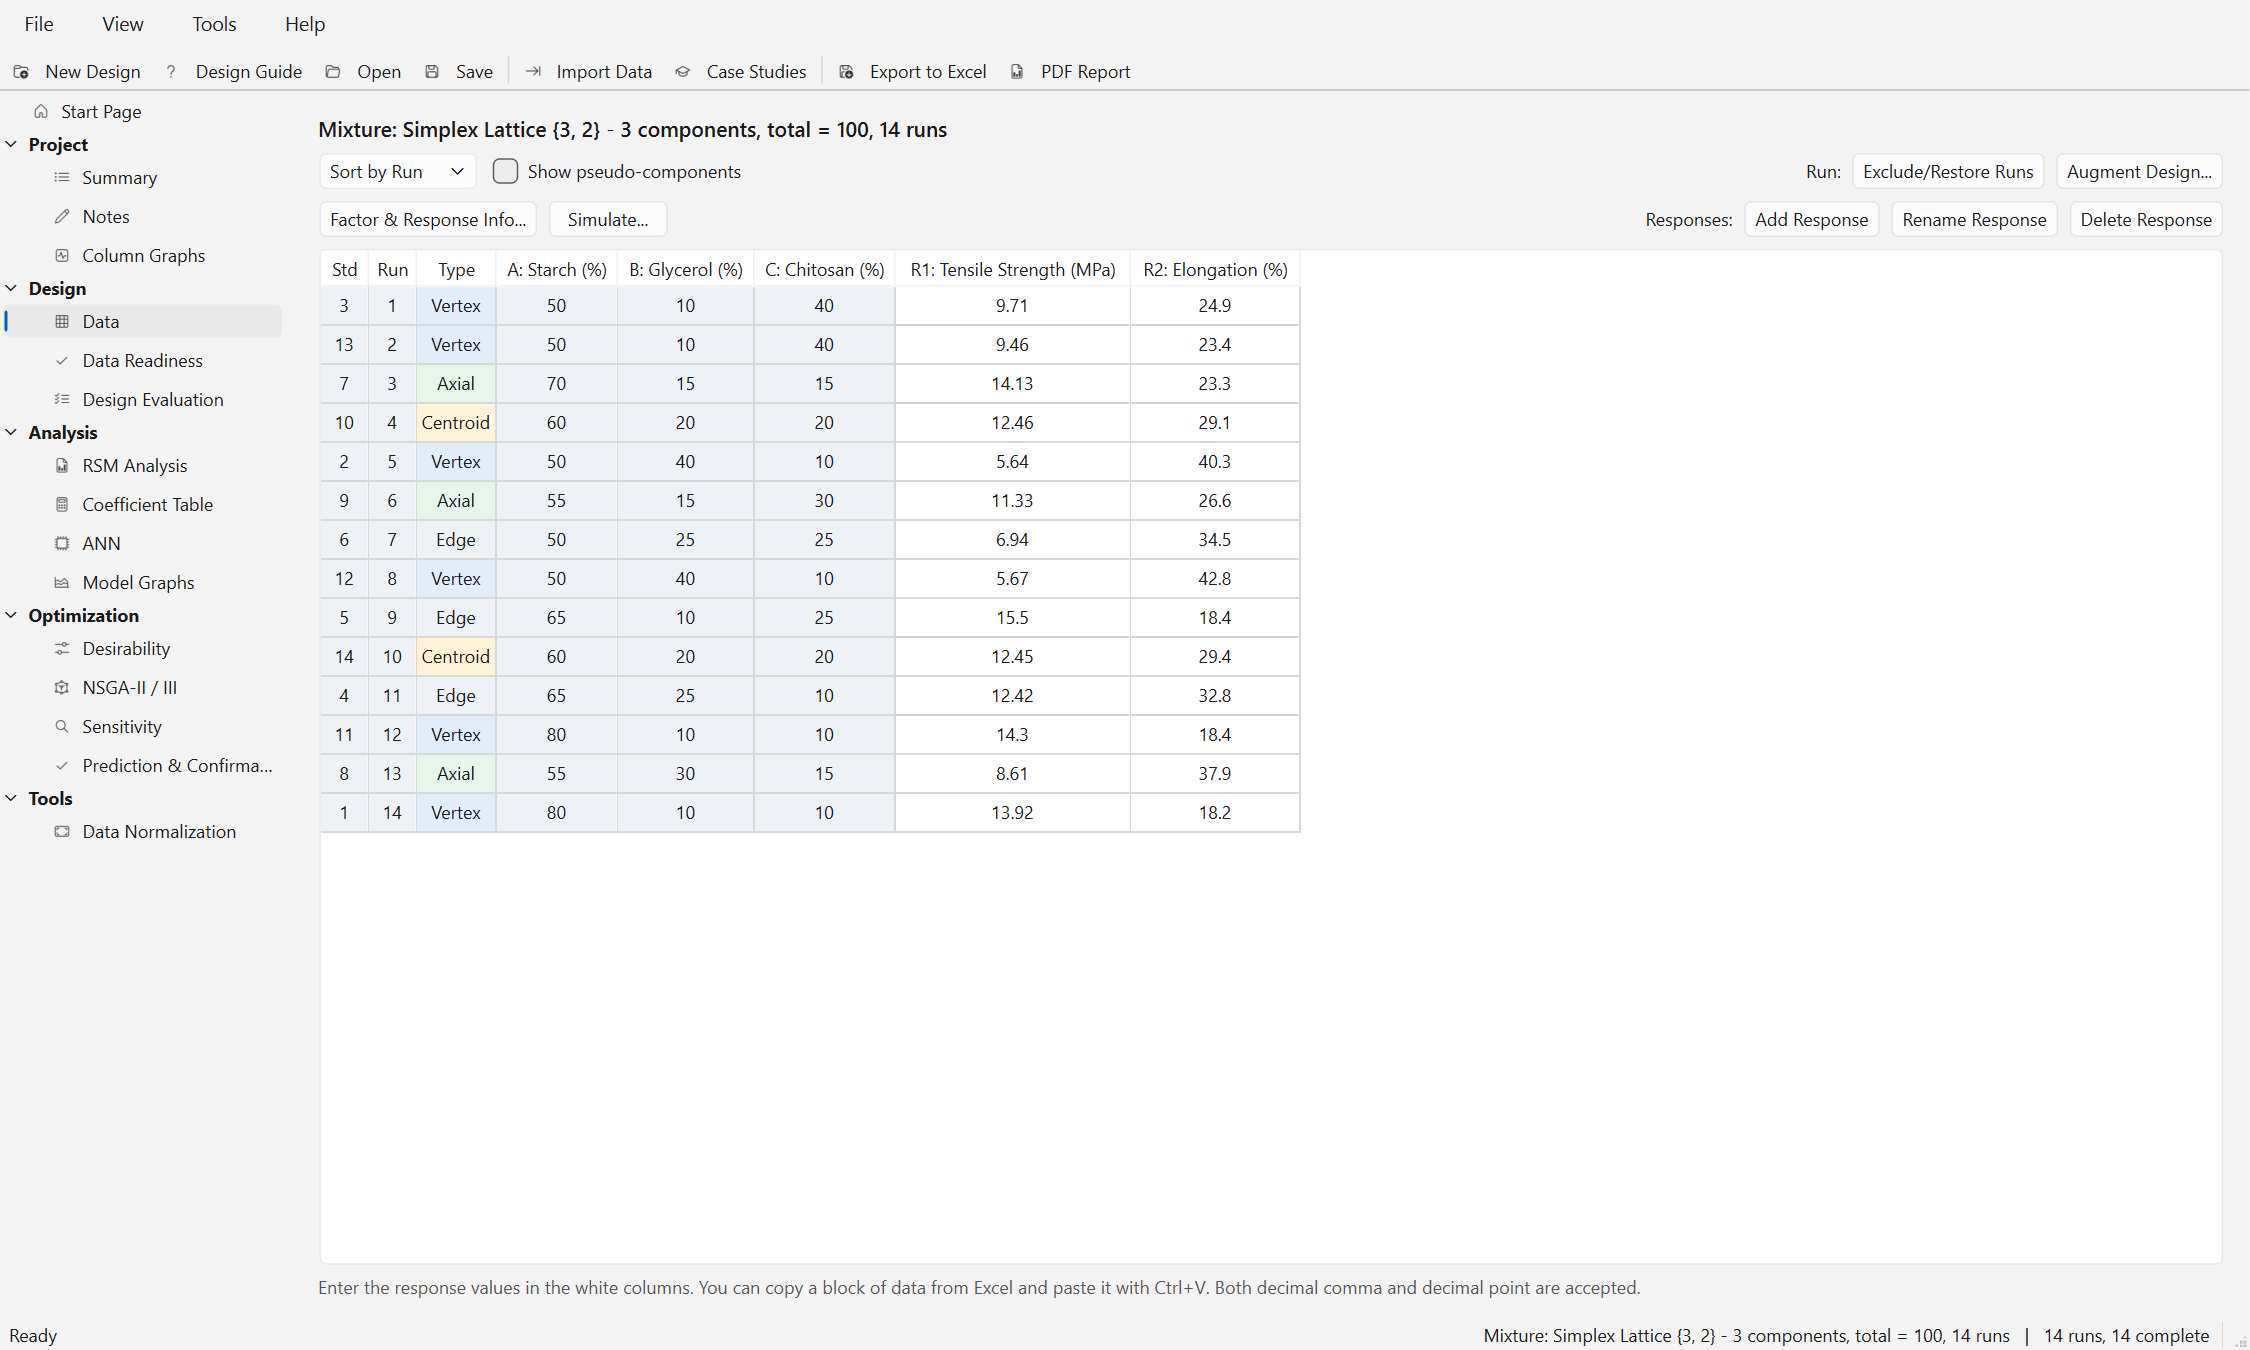
\includegraphics[width=\linewidth]{data_mixture.png}
\caption{Data page of the mixture case ``Edible Film Formulation (Mixture)'': simplex lattice \{3, 2\}, total 100,
14 runs with colour-coded point types.}
\label{fig:ch04-datamix}
\end{figure}

\begin{figure}[htbp]
\centering
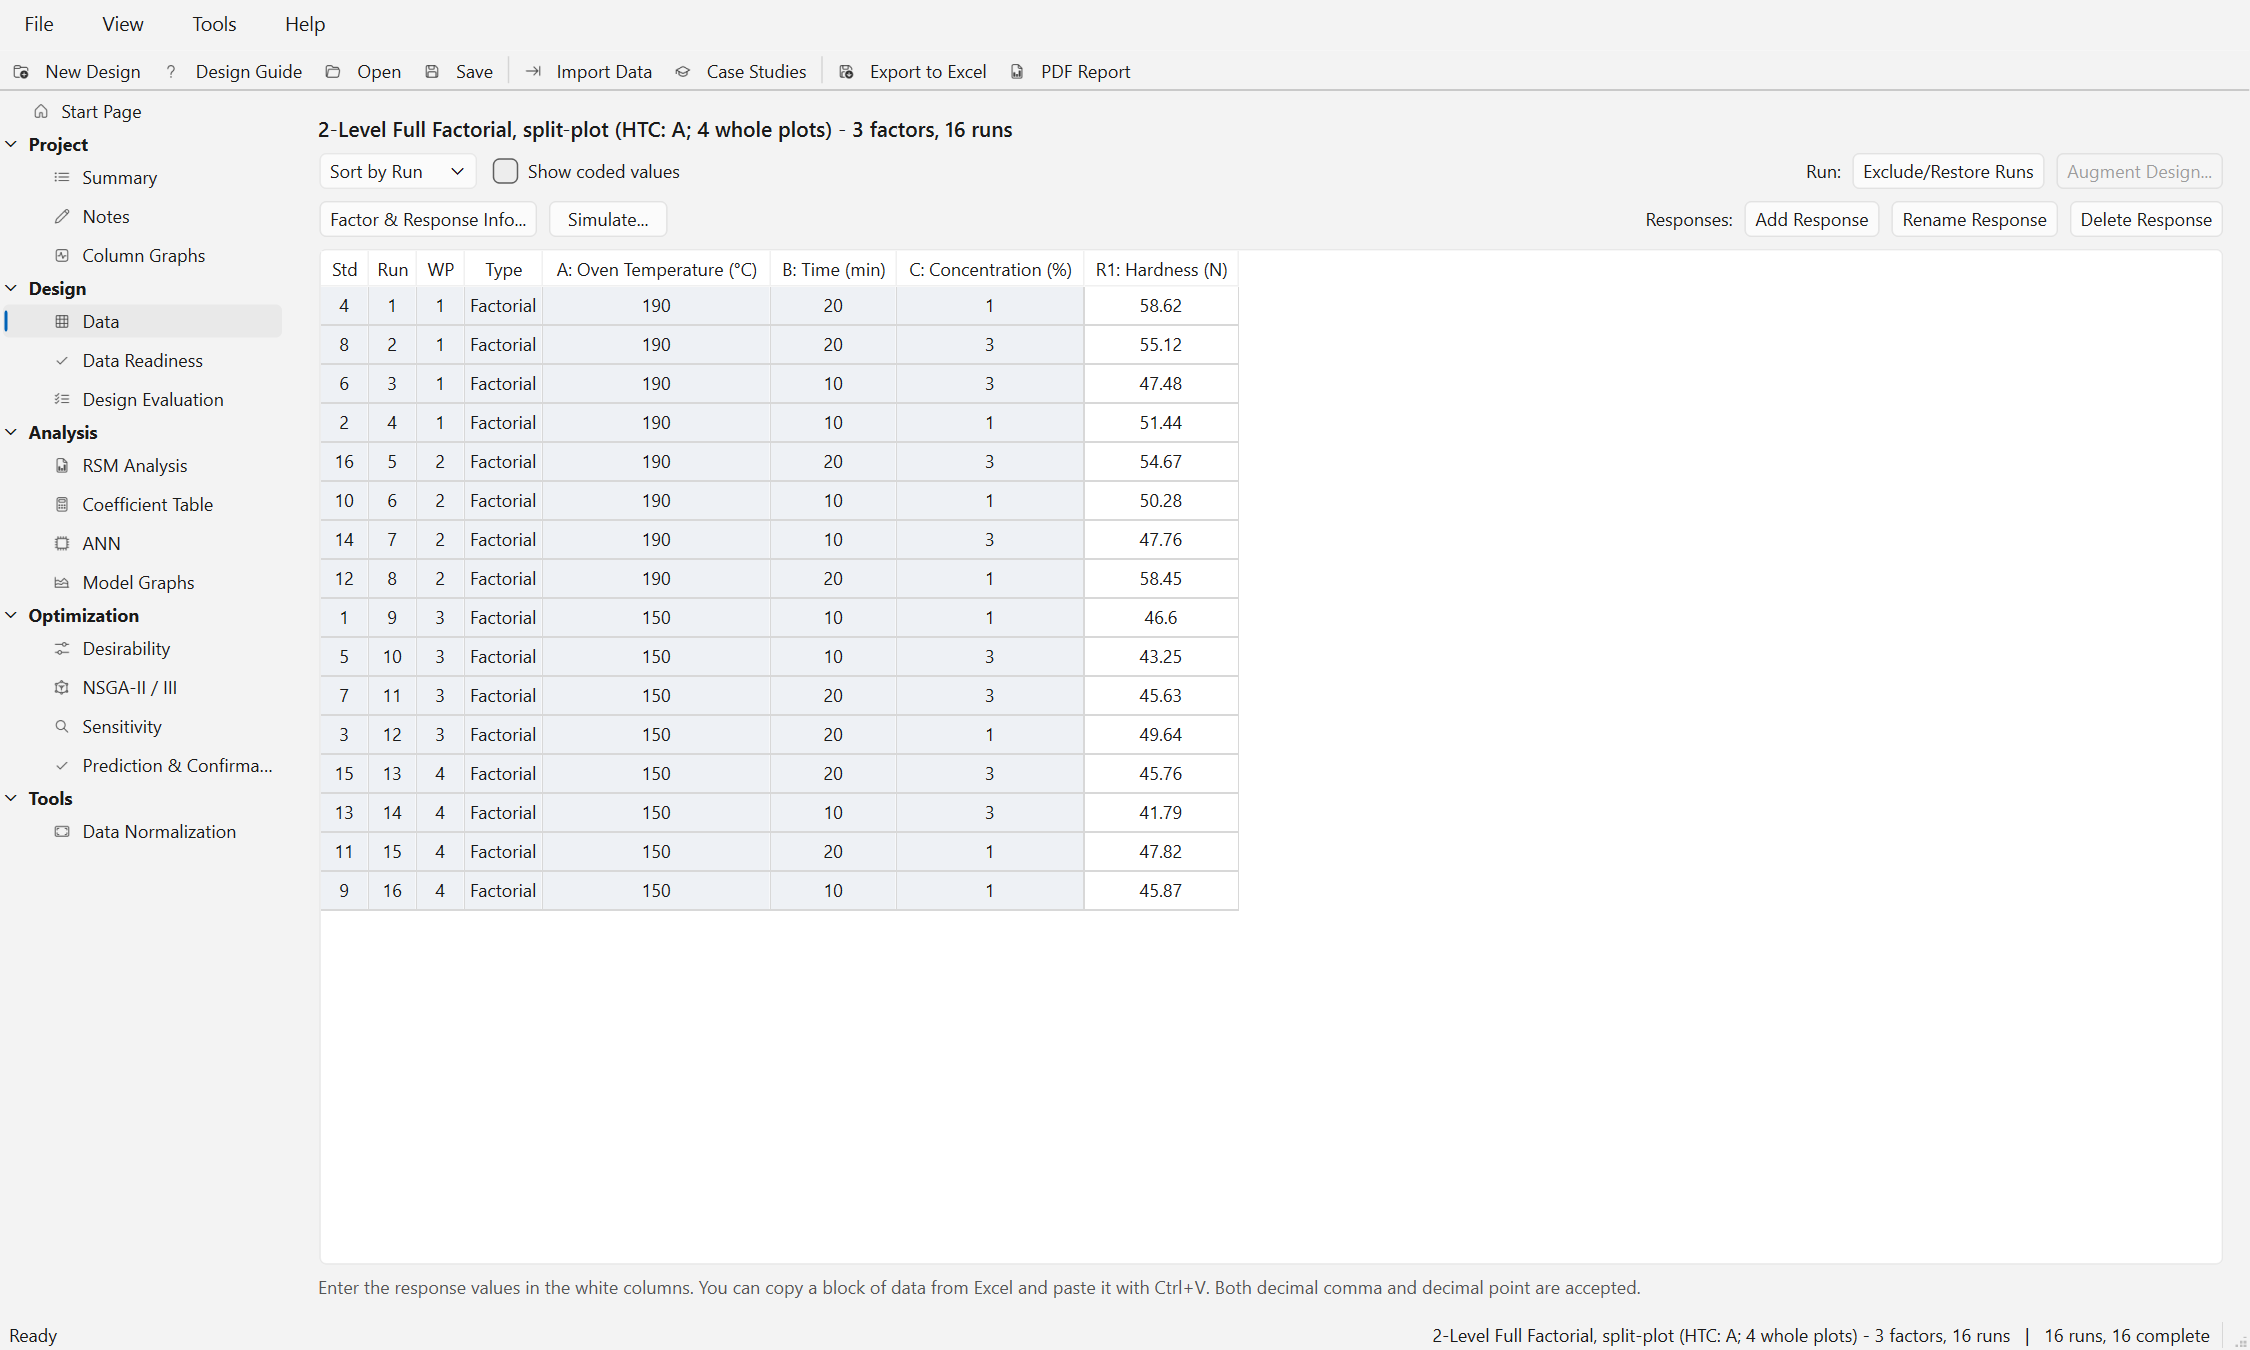
\includegraphics[width=\linewidth]{data_splitplot.png}
\caption{Data page of the split-plot case ``Oven Product Hardness (Split-Plot)'': column WP (whole plot); the
hard-to-change Oven Temperature is constant within each whole plot.}
\label{fig:ch04-datasplit}
\end{figure}

\section{Factor \& Response Info}
\label{sec:ch04-info}

\paragraph{Purpose.} This dialog stores the information about factors and responses that is not part of the design
itself: the standard deviation of each factor for propagation of error (POE), and the type of each response.

\paragraph{How to use.} Click \ui{Factor \& Response Info\dots} on the Data page, edit the tables and click
\ui{Save}.

\begin{table}[htbp]
\centering
\caption{Fields of the Factor \& Response Info dialog.}
\label{tab:ch04-info}
\small
\begin{tabularx}{\linewidth}{@{}p{3.6cm}p{3.6cm}X@{}}
\toprule
Field & Values & Meaning \\
\midrule
\ui{Standard deviation ($\sigma$)} & number $\ge 0$ or empty & Standard deviation of the factor setting in actual
units (how precisely the factor can be held). Empty = controlled precisely. Not available for categorical
factors. \\
\ui{Name}, \ui{Unit} & text & Name and unit of the response. \\
\ui{Type} & Normal (continuous), Binomial (successes out of n), Poisson (counts) & Distribution of the response;
selects the analysis (least squares, logistic regression or Poisson regression). \\
\ui{Trials per run} & number $\ge 1$ & Number of trials $n$ per run for a binomial response (required). \\
\bottomrule
\end{tabularx}
\end{table}

\paragraph{Theory.} POE uses the standard deviations in coded units,
\begin{equation}
\sigma_{\text{coded}} = \frac{\sigma}{s}, \qquad s = \frac{H-L}{2} \ \text{(process factor)}, \quad
s = T - \textstyle\sum_j L_j \ \text{(mixture component)},
\label{eq:ch04-sdcoded}
\end{equation}
where $s$ is the scale of Equation~(\ref{eq:ch03-coding}) or (\ref{eq:ch03-pseudo}). For the extraction case with
$\sigma = 1.0$ \textdegree C, 2.0 min and 0.05 \% the coded values are 0.1, 0.0667 and 0.05. The POE graph and the
POE criterion of the optimization become available once at least one $\sigma$ is entered (Chapters~6 and 8).

A \emph{binomial} response is the number of successes out of $n$ trials per run (for example germinated seeds out of
50) and is analyzed by logistic regression; a \emph{Poisson} response is a count of events and is analyzed by
Poisson regression (Chapter~\ref{chap:5}). Changing the type of a response resets its model specification. Messages: ``The
standard deviation of X is not a number.'' and ``Enter the number of trials per run for X.''. Negative values are
ignored.

\begin{figure}[htbp]
\centering
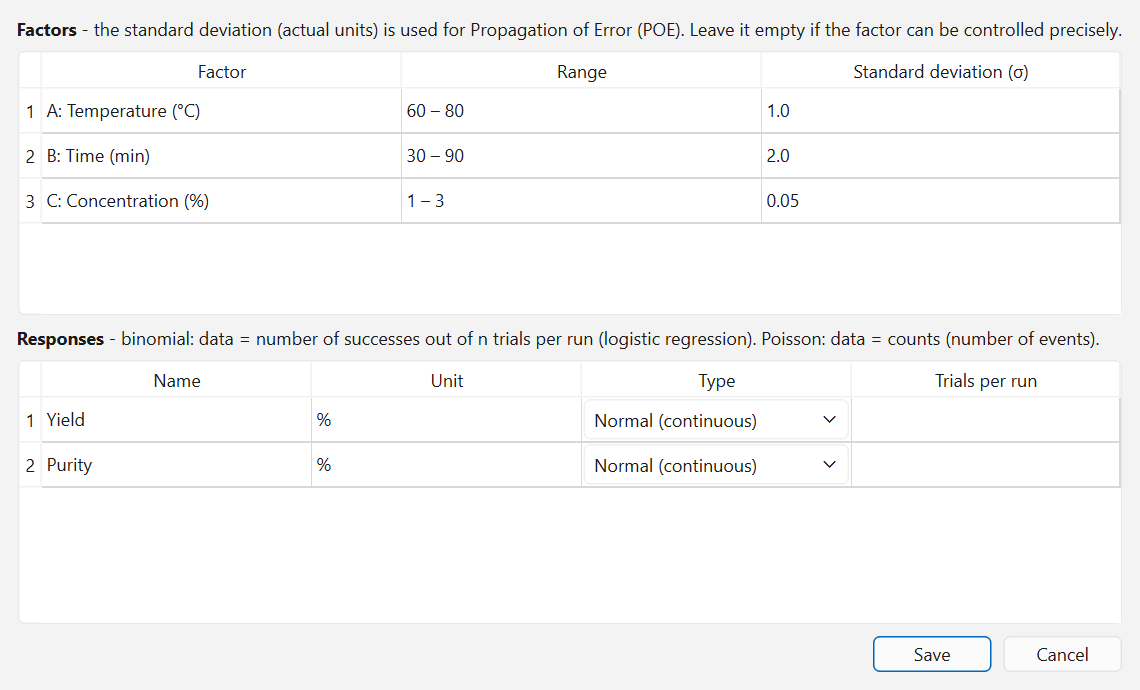
\includegraphics[width=0.75\linewidth]{factor_response_info.png}
\caption{Factor \& Response Info dialog for the extraction case with $\sigma$ = 1.0 \textdegree C (Temperature),
2.0 min (Time) and 0.05 \% (Concentration).}
\label{fig:ch04-info}
\end{figure}

\section{Simulate Response}
\label{sec:ch04-simulate}

\paragraph{Purpose.} \ui{Simulate\dots} fills a response column from an equation plus random noise. It is used for
practice and teaching, for checking how well a design recovers a known model before running it, and for testing the
analysis.

\paragraph{How to use.}
\begin{enumerate}
\item Click \ui{Simulate\dots} on the Data page.
\item Choose the \ui{Response:}, type the \ui{Equation:}, choose the \ui{Factor units:} and set \ui{Noise
($\sigma$):} and \ui{Random seed:}.
\item Tick \ui{Fill empty cells only} to keep values that are already entered.
\item Click \ui{Simulate}. The message ``n response values filled.'' reports the number of cells written.
\end{enumerate}

\begin{table}[htbp]
\centering
\caption{Options of the Simulate Response dialog.}
\label{tab:ch04-simopts}
\small
\begin{tabularx}{\linewidth}{@{}p{3.0cm}p{4.4cm}p{2.4cm}X@{}}
\toprule
Option & Values & Default & Meaning \\
\midrule
\ui{Equation:} & expression (Table~\ref{tab:ch04-simsyntax}) & \texttt{50 + 3*A - 2*B - 4*A**2} & mean response \\
\ui{Factor units:} & Coded factors (-1..+1 / pseudo-components), Actual factors & Coded & scale of the letters \\
\ui{Noise ($\sigma$):} & 0--10\textsuperscript{9} & 1.0 & standard deviation of normal noise \\
\ui{Random seed:} & 0--999\,999 & 1 & same seed = same noise \\
\ui{Fill empty cells only} & check box & off & keep existing values \\
\bottomrule
\end{tabularx}
\end{table}

\paragraph{Equation syntax.} The equation is evaluated safely: only the elements of
Table~\ref{tab:ch04-simsyntax} are allowed.

\begin{table}[htbp]
\centering
\caption{Elements accepted in a simulation equation.}
\label{tab:ch04-simsyntax}
\small
\begin{tabularx}{\linewidth}{@{}p{3.2cm}X@{}}
\toprule
Element & Accepted \\
\midrule
Variables & factor letters A, B, C, \dots{} (I is skipped). Categorical factors take their level index 0, 1, 2, \dots \\
Numbers & with a point as the decimal separator, e.g.\ \texttt{2.5} \\
Operators & \texttt{+ - * /}, power \texttt{**} or \texttt{\textasciicircum}, remainder \texttt{\%} \\
Comparisons & \texttt{< > <= >= == !=}; true = 1, false = 0, e.g.\ \texttt{5*(A > 0)} \\
Functions & \texttt{exp}, \texttt{ln}, \texttt{log} (natural log), \texttt{log10}, \texttt{sqrt}, \texttt{sin},
\texttt{cos}, \texttt{tan}, \texttt{abs} (one argument); \texttt{min(a, b)}, \texttt{max(a, b)} (two arguments) \\
Constants & \texttt{pi}, \texttt{e} \\
Comma & only between the two arguments of \texttt{min} and \texttt{max} \\
\bottomrule
\end{tabularx}
\end{table}

Typical errors: ``Invalid equation: \dots'' (a syntax error; when the text contains a comma the note ``Use a point as
the decimal separator (for example 2.5); commas only separate the arguments of min and max.'' is added), ``Unknown
name 'x'. Use the factor letters (A, B, ...).'', ``Only basic math functions are allowed.'' and ``min() takes 2
arguments.''.

\paragraph{Theory.} Let $f(x)$ be the value of the equation for a run. Depending on the response type:
\begin{align}
\text{Normal:}\quad & y = f(x) + \varepsilon, \quad \varepsilon \sim N(0, \sigma^2), \label{eq:ch04-simnorm}\\
\text{Binomial:}\quad & y \sim \text{Bin}\bigl(n, \operatorname{clip}(f(x), 0, 1)\bigr), \label{eq:ch04-simbin}\\
\text{Poisson:}\quad & y \sim \text{Pois}\bigl(\max(f(x), 0)\bigr). \label{eq:ch04-simpois}
\end{align}
For a binomial response the equation is the success probability, for a Poisson response the mean count. The noise
$\sigma$ applies to normal responses only: for binomial and Poisson responses the field is disabled with the note
``Not used: binomial and Poisson data get their random variation from the distribution.'' Only runs with complete
factor values are filled.

\paragraph{Example.} On a new rotatable CCD with three factors (20 runs), the default equation with coded factors and
$\sigma = 1$ fills all 20 Yield values (``20 response values filled.''). Fitting a quadratic model should then
recover coefficients close to 3, $-2$ and $-4$ for A, B and A\textsuperscript{2}, within about two standard errors
(Design Evaluation gives the standard errors in units of $\sigma$; Section~\ref{sec:ch04-eval}).

\begin{figure}[htbp]
\centering
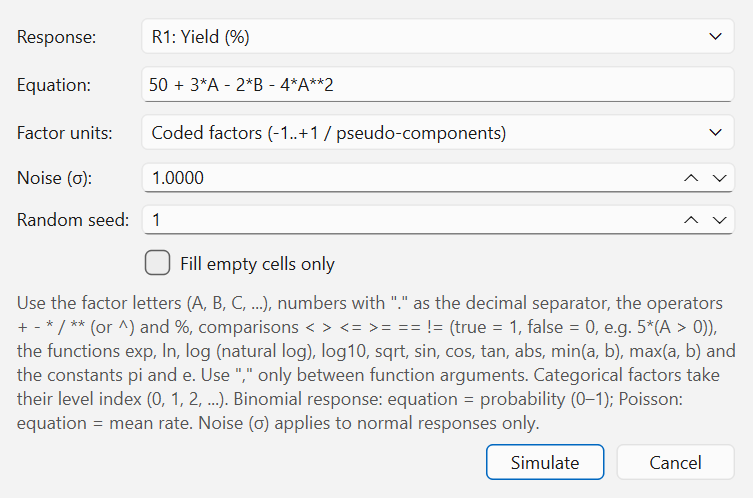
\includegraphics[width=0.6\linewidth]{simulate_dialog.png}
\caption{Simulate Response dialog with the default equation, coded factors, noise $\sigma$ = 1 and seed 1.}
\label{fig:ch04-simulate}
\end{figure}

\section{Data Readiness}
\label{sec:ch04-readiness}

\paragraph{Purpose.} The \ui{Data Readiness} page answers the question ``Are these data good enough to build a
model and to trust an optimum, and if not, what should be done?''. It runs a set of checks on one response, scores
them, lists recommendations (complete the data, or treat the data or the model), and computes suggested additional
runs that can be added to the data sheet with one click. It is especially useful for historical data, which were not
collected according to a design.

\subsection{How to use}
\begin{enumerate}
\item Open \ui{Data Readiness} in the group \ui{Design}.
\item Select the \ui{Response:} and the \ui{Reference model:} (by default the model currently selected for that
response). Click \ui{Reassess} after changing the data elsewhere.
\item Read the score cards, the report on the left and the recommendation list on the right.
\item Select a recommendation and click \ui{Apply Selected Recommendation}. Recommendations marked ``(manual)'' must
be carried out by you; REGEN shows their text.
\item Choose a set of suggested runs under \ui{Suggested runs:}, inspect the table (factor settings in actual units
and, when a model exists, the predicted response) and click \ui{Add Suggested Runs to Data Sheet}. Perform these
experiments, then enter their responses on the Data page.
\end{enumerate}

\subsection{Output}
The six score cards are \ui{Modeling}, \ui{Optimization} and one per category: \ui{Data Completeness \&
Cleanliness}, \ui{Data Structure for Modeling}, \ui{Response \& Model Quality} and \ui{Optimization Readiness}. The
two overall cards show the verdict; the category cards show ``good'' or the number of notes (checks that need
attention or have a problem). The report starts, for projects with more than one response, with a ``Readiness
Summary for All Responses'' table, followed by the verdicts, the number of complete runs and the reference model, one
table per category (Check, Value, Status, Explanation) and the table of recommendations. The status of a check is
\emph{Good}, \emph{Needs attention}, \emph{Problem} or \emph{Info}.

\subsection{Scores and verdicts}
Each check is rated $w = 1$ (Good), $0.5$ (Needs attention) or $0$ (Problem); Info checks are not counted. The score
of a category $c$ with $m_c$ rated checks is
\begin{equation}
S_c = \frac{100}{m_c} \sum_{i \in c} w_i .
\label{eq:ch04-score}
\end{equation}
The modeling score is the mean of the available scores of the categories data, structure and response quality; the
optimization score is the mean of all four category scores (including optimization readiness). The verdict is
\begin{equation}
\text{verdict} = \begin{cases}
\text{``Ready''} & S \ge 85,\\
\text{``Fair - some things need fixing''} & 60 \le S < 85,\\
\text{``Not ready yet''} & S < 60,\\
\text{``Cannot be assessed yet''} & \text{no score.}
\end{cases}
\label{eq:ch04-verdict}
\end{equation}
The thresholds are practical choices, not statistical tests: a score summarizes how many checks pass, it does not
replace reading the individual checks. Recommendations are sorted by the status of their check (problems first)
and, within a status, data completion before treatment.

\subsection{The checks}
Let $N$ be the number of runs with complete factors and a response value (excluded runs count as empty), $p$ the
number of parameters of the reference model and $\nu = N - p$ the residual degrees of freedom. If $N < 3$ the
assessment stops after the first check. Table~\ref{tab:ch04-checks} lists all checks with their rules. Some checks
apply only to normally distributed responses fitted by least squares, some only to process (non-mixture) designs.

\begin{longtable}{@{}p{3.1cm}p{5.6cm}p{6.1cm}@{}}
\caption{Checks of the Data Readiness assessment.}\label{tab:ch04-checks}\\
\toprule
Check & Status rule & Recommendation (action) \\
\midrule
\endfirsthead
\toprule
Check & Status rule & Recommendation (action) \\
\midrule
\endhead
\multicolumn{3}{@{}l}{\emph{Data Completeness \& Cleanliness}}\\
Missing data & Good if no empty factor or response cell; Problem if $N < 3$; else Needs attention &
  Fill in or delete incomplete rows; perform the missing runs (manual). \\
Exact duplicate rows & Needs attention if rows have identical factors \emph{and} response &
  Check them; delete rows that were recorded twice (manual). True replicates almost never give identical values. \\
Constant factors & Problem if a numeric factor has the same value in every run & Remove the factor or add runs at
  other levels (manual). \\
\midrule
\multicolumn{3}{@{}l}{\emph{Data Structure for Modeling}}\\
Runs vs model parameters & Good $\nu \ge 5$; Needs attention $1 \le \nu < 5$; Problem $\nu \le 0$ &
  Add $\max(0, p + 5 - N)$ D-optimal runs. \\
Numeric factor levels (process designs) & Good if every numeric factor has $\ge 3$ distinct levels; otherwise
  Problem if the model has squared terms, else Needs attention & Add $\max(3, 2 \times \text{number of 2-level
  factors})$ D-optimal runs for the quadratic model (``Middle level (curvature)''). \\
Replicates (pure error) & Good if pure-error df $\ge 3$; Needs attention 1--2; Problem 0 & Add 4 replicates at the
  center (mixtures: the centroid of the mixture region). \\
Multicollinearity (max VIF) & Good $\le 5$; Needs attention $\le 10$; Problem $> 10$ & Add
  $\max(4, \lfloor p/2 \rfloor)$ D-optimal runs. \\
High-leverage points & Needs attention if any $h_i > \max(2p/N, 0.5)$ & Add $\max(5, \min(20, \lfloor N/4
  \rfloor))$ gap-filling runs around them. \\
Factor space coverage (process designs) & Good $g \le 0.3$; Needs attention $\le 0.5$; Problem $> 0.5$ & Add
  gap-filling runs. \\
Level balance of \textless factor\textgreater{} (each categorical factor) & Good if the rarest level has $\ge
  \max(3, 0.5 \times \text{most frequent})$ runs; Needs attention if $\ge 2$; else Problem & Add runs at the rarest
  level (manual). \\
\midrule
\multicolumn{3}{@{}l}{\emph{Response \& Model Quality} (normal responses)}\\
Outliers \& influential points & Needs attention if any outlier or Cook's $D > 1$ & Exclude those runs after
  checking them. \\
Response spread \& transform & Needs attention if Box-Cox recommends a transform, none is in use and the residual
  SS drops by $\ge 5\,\%$ & Apply the recommended transform. \\
Constant residual variance ($N > 5$) & Needs attention if Spearman $\rho(|e|, \hat y) > 0$ with $p < 0.05$ & Use a
  ln transform ($y > 0$) or square root. \\
Drift over run order & Needs attention if $DW < 1.4$ or $DW > 2.6$ or the trend has $p < 0.01$ & Check
  calibration and materials, use blocks, randomize (manual). \\
Model fit & Needs attention if lack of fit $p < 0.05$, or Adj R\textsuperscript{2} $-$ Pred R\textsuperscript{2}
  $> 0.2$, or Pred R\textsuperscript{2} $< 0.5$; Problem if Pred R\textsuperscript{2} $< 0$; Info ``R², Adj R², Pred
  R² not available'' for split-plot (REML) responses & Higher-order model; backward elimination with $\alpha = 0.10$
  (split-plot: judge the model by the Wald F tests on the Split-Plot (REML) tab). \\
Signal / noise (needs pure error) & Good $\ge 4$; Needs attention $\ge 2$; Problem $< 2$ & Improve precision,
  average repeats or widen the ranges (manual). \\
Model & Problem if the model cannot be calculated & (error text) \\
\midrule
\multicolumn{3}{@{}l}{\emph{Optimization Readiness}}\\
Model significance & Good if the model $p < 0.05$, else Problem; Info ``no overall model F test (split-plot)'' for
  split-plot (REML) responses & Add runs or widen the factor ranges (manual). \\
Prediction reliability (Pred R\textsuperscript{2}) & Good $\ge 0.7$; Needs attention $\ge 0.4$; Problem $< 0.4$ &
  Add D-optimal runs; with $N \ge 30$ also ``try an ANN'' (manual). \\
Optimum location & Needs attention if a process factor of the optimum lies within 2\,\% of its range from a bound
  & Extend the range in that direction (steepest ascent) (manual). \\
Data support around the optimum & Needs attention if $d > 0.2$ or the CI half-width exceeds 10\,\% of the response
  range & 4 confirmation runs around the optimum. \\
\bottomrule
\end{longtable}

\subsection{Formulas as implemented}
\paragraph{Outliers.} A run is an outlier if its externally studentized residual exceeds the Bonferroni limit,
\begin{equation}
|t_i| > t_{1 - 0.05/(2N),\; \nu - 1},
\label{eq:ch04-bonf}
\end{equation}
and it is influential if Cook's distance $D_i > 1$ \citep{cook1977}. Both are explained in Chapter~\ref{chap:5}.

\paragraph{Box-Cox.} The residual sum of squares of the scaled power transform
$w = (y^\lambda - 1)/(\lambda \dot y^{\lambda-1})$ ($w = \dot y \ln y$ for $\lambda = 0$, $\dot y$ = geometric mean)
is computed for 121 values $\lambda \in [-3, 3]$ \citep{boxcox1964}. The 95\,\% interval contains all $\lambda$ with
$\ln SS(\lambda) \le \ln SS_{\min} + \ln(1 + t^2_{0.975,\nu}/\nu)$. No transform is recommended if $\lambda = 1$
lies inside; otherwise the first of square root ($\lambda = 0.5$), ln (0) and inverse ($-1$) inside the interval, or
the power transform with the best $\lambda$. The gain is $1 - \exp(\ln SS_{\min} - \ln SS(1))$.

\paragraph{Constant variance and drift.} The variance check uses the Spearman rank correlation \citep{spearman1904}
between $|e_i|$ and $\hat y_i$. For drift the residuals are sorted by run order and the Durbin--Watson statistic
\citep{durbin1950}
\begin{equation}
DW = \frac{\sum_{t=2}^{N} (e_t - e_{t-1})^2}{\sum_{t=1}^{N} e_t^2}
\label{eq:ch04-dw}
\end{equation}
is computed ($DW \approx 2$ for independent residuals); the trend is the Spearman correlation between run order and
residual.

\paragraph{Signal to noise.} With $SS_{PE}$ and $df_{PE}$ the pure-error sum of squares and degrees of freedom of
replicated points (identical coded settings, same block),
\begin{equation}
\text{SNR} = \frac{\operatorname{SD}(y)}{\sqrt{SS_{PE}/df_{PE}}} .
\label{eq:ch04-snr}
\end{equation}

\paragraph{Coverage gap.} Numeric factors are scaled to $[0,1]$ by their coded bounds ($u$), 3000 points $u_r$ are
drawn from the design region (respecting constraints), and
\begin{equation}
g = \frac{1}{\sqrt{k_{\text{num}}}}\, \max_r \min_i \lVert u_r - u_i \rVert ,
\label{eq:ch04-gap}
\end{equation}
the largest distance from a point of the region to the nearest run, relative to the diagonal of the unit cube.

\paragraph{Optimum.} The optimum is the first solution of the last desirability optimization if one exists (``last
optimization result''), otherwise the best of 4000 random region points according to the goal of the response in the
optimization criteria (default maximize: ``Model-predicted maximum''). The distance $d$ to the nearest run is
computed like Equation~(\ref{eq:ch04-gap}); $h$ is the half-width of the model's 95\,\% confidence interval at the
optimum.

\subsection{Suggested runs}
\label{sec:ch04-suggest}
\begin{itemize}
\item \emph{D-optimal (adds model information)} and \emph{Middle level (curvature)}: 3000 random points of the region
are the candidates. Runs are added one at a time, each time the candidate with the largest prediction variance
$x^\top M^{-1} x$, with $M = X_e^\top X_e + 10^{-6} I$ for the existing runs, updated by Sherman--Morrison:
\begin{equation}
M^{-1} \leftarrow M^{-1} - \frac{M^{-1} x x^\top M^{-1}}{1 + x^\top M^{-1} x}.
\label{eq:ch04-sm}
\end{equation}
Adding the point of largest prediction variance gives the largest increase of $\det M$, so this is a greedy
D-optimal augmentation \citep{goos2011}.
\item \emph{Factor space gap filling}: from 3000 region points, repeatedly the point farthest from all existing and
already chosen runs (maximin), with numeric factors scaled to $[0,1]$.
\item \emph{Replicates (pure error)}: 4 copies of the center point (mixtures: the overall centroid of the mixture
region; categorical factors from the run nearest the center).
\item \emph{Confirmation around the optimum}: the optimum itself and up to three random region points within a
scaled distance of 0.15 from it, with the same categorical levels.
\end{itemize}
The confirmation ``Add n runs (\textless label\textgreater) to the data sheet? Their responses are empty and must be
entered after the experiments are run.'' precedes the addition. The runs are added with the point types D-optimal,
Mid-level, Replicate, Space-filling or Confirmation, at the end of the run order; in split-plot designs each new run
forms its own whole plot. The suggestions use fixed random seeds, so a reassessment of the same data gives the same
suggestions.

\paragraph{Apply Selected Recommendation.} Depending on the recommendation: suggested runs are added (as above); runs
are excluded after the question ``Ignore runs \dots{} in the analysis? The data are not deleted and can be restored on
the Data or Diagnostics page.''; or the model specification of the response is changed (transform, higher model
order, or backward elimination at $\alpha_{\text{out}} = 0.10$) and the page is reassessed.

\subsection{Examples}
\paragraph{A good designed experiment.} For the BBD extraction case, response Yield, quadratic reference model
(Figure~\ref{fig:ch04-readiness}), the modeling score is 94 and the optimization score 96, both ``Ready''. All
structure checks are Good (17 runs, 10 parameters, residual df 7; 3 levels per factor; pure-error df 4; max VIF 1.01;
largest gap 0.27). Two checks need attention: ``0 outliers, 2 Cook's $>$ 1'' (runs 1 and 7) and the model fit with
lack-of-fit $p = 0.030$; the recommendations are to check runs 1 and 7 and to try a higher-order model, a transform
or an ANN. The optimum predicted by the model (Temperature 75.5 \textdegree C, Time 86.1 min, Concentration 2.30 \%)
lies 0.16 from the nearest run with a CI of $\pm 0.99$ (7\,\% of the range), so the only suggested runs are four
confirmation runs. Purity scores 100 and 97; its optimum is less well supported (CI 10\,\% of the range).

\begin{figure}[htbp]
\centering
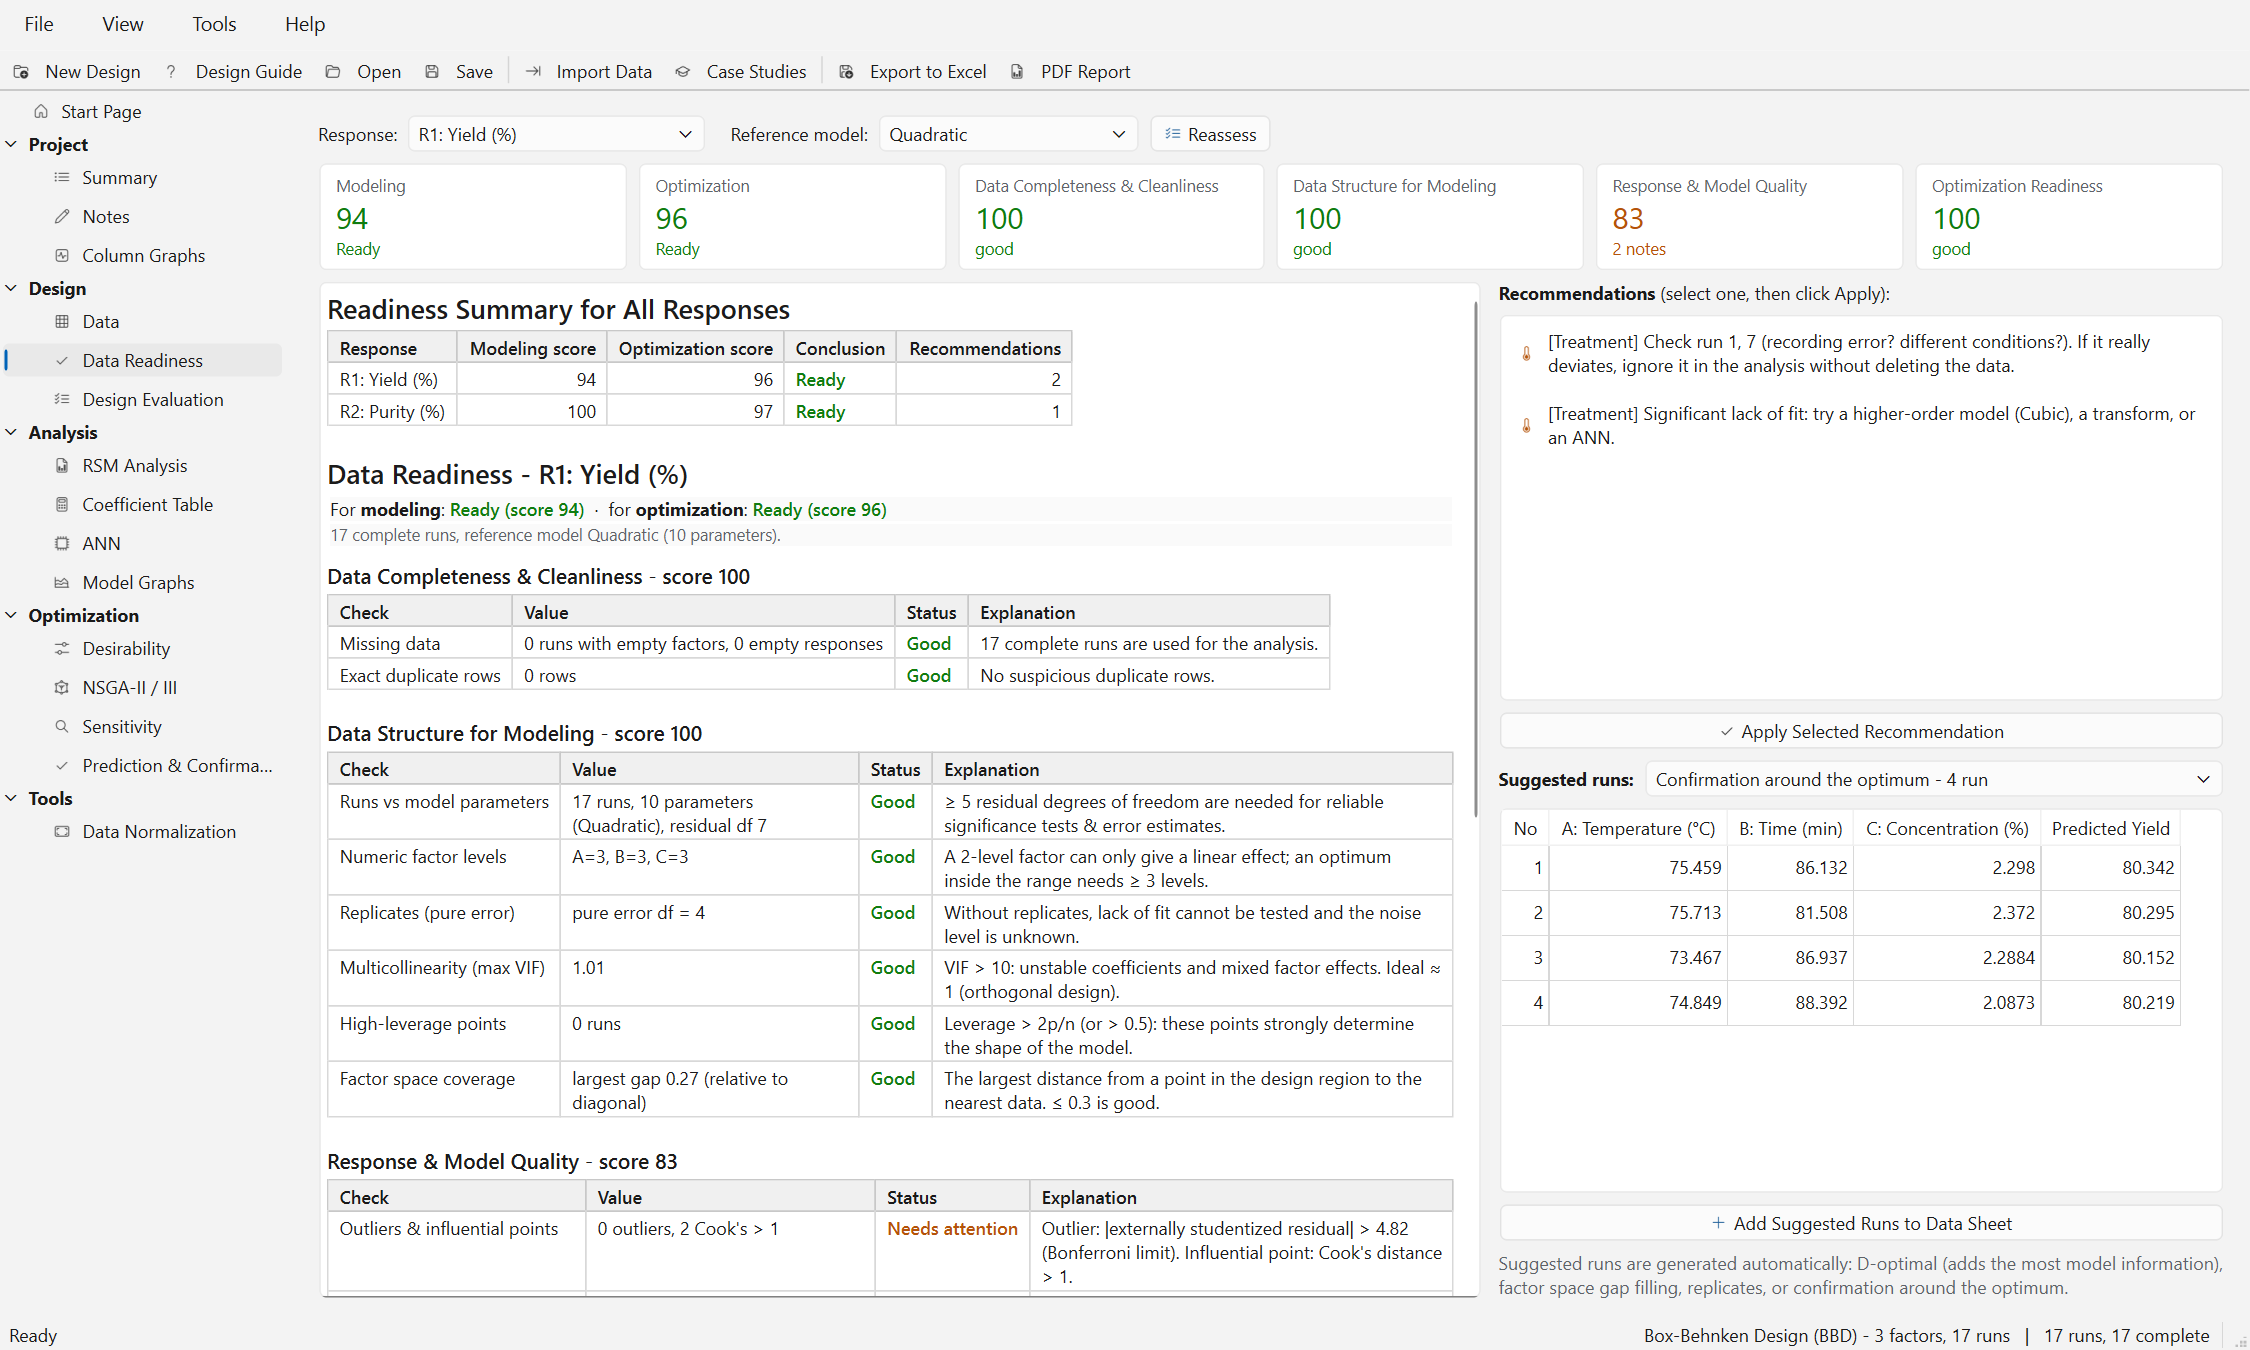
\includegraphics[width=\linewidth]{readiness.png}
\caption{Data Readiness of the BBD extraction case, response Yield: Modeling 94 and Optimization 96 (Ready), two
notes in Response \& Model Quality, and four suggested confirmation runs around the optimum.}
\label{fig:ch04-readiness}
\end{figure}

\paragraph{Historical data for an ANN.} The dye adsorption case (40 Latin hypercube runs, quadratic reference model
with 15 parameters; Figure~\ref{fig:ch04-readinessdye}) scores 82 for modeling and 77 for optimization (``Fair -
some things need fixing''). The category scores follow Equation~(\ref{eq:ch04-score}): Data Structure 75
($[1 + 1 + 0 + 1 + 0.5 + 1]/6$, with ``pure error df = 0'' a Problem and one high-leverage run), Response \& Model
Quality 70 and Optimization Readiness 62.5 (shown as 62). The findings: no replicates; Box-Cox $\lambda = 0.00$ (CI
$-0.15$ to $0.15$) with an 87\,\% drop of the residual SS, so a ln transform is recommended; Durbin--Watson 1.36
(possible drift); Pred R\textsuperscript{2} 0.562; the predicted optimum has Adsorbent Dose 0.53 g/L, within 2\,\%
of its lower limit 0.5, and a CI of $\pm 17.8$ (32\,\% of the range). Suggested runs: 4 replicates at pH 6, dose
2.25 g/L, time 65 min, concentration 110 mg/L; 10 gap-filling runs; 7 D-optimal runs; 4 confirmation runs. Because
$N \ge 30$ and Pred R\textsuperscript{2} is low, an ANN is also suggested. A sensible order of action is: add the
replicates (they also make the ANN diagnosis possible), apply the ln transform, reassess, then compare RSM with an
ANN (Chapter~\ref{chap:7}).

\begin{figure}[htbp]
\centering
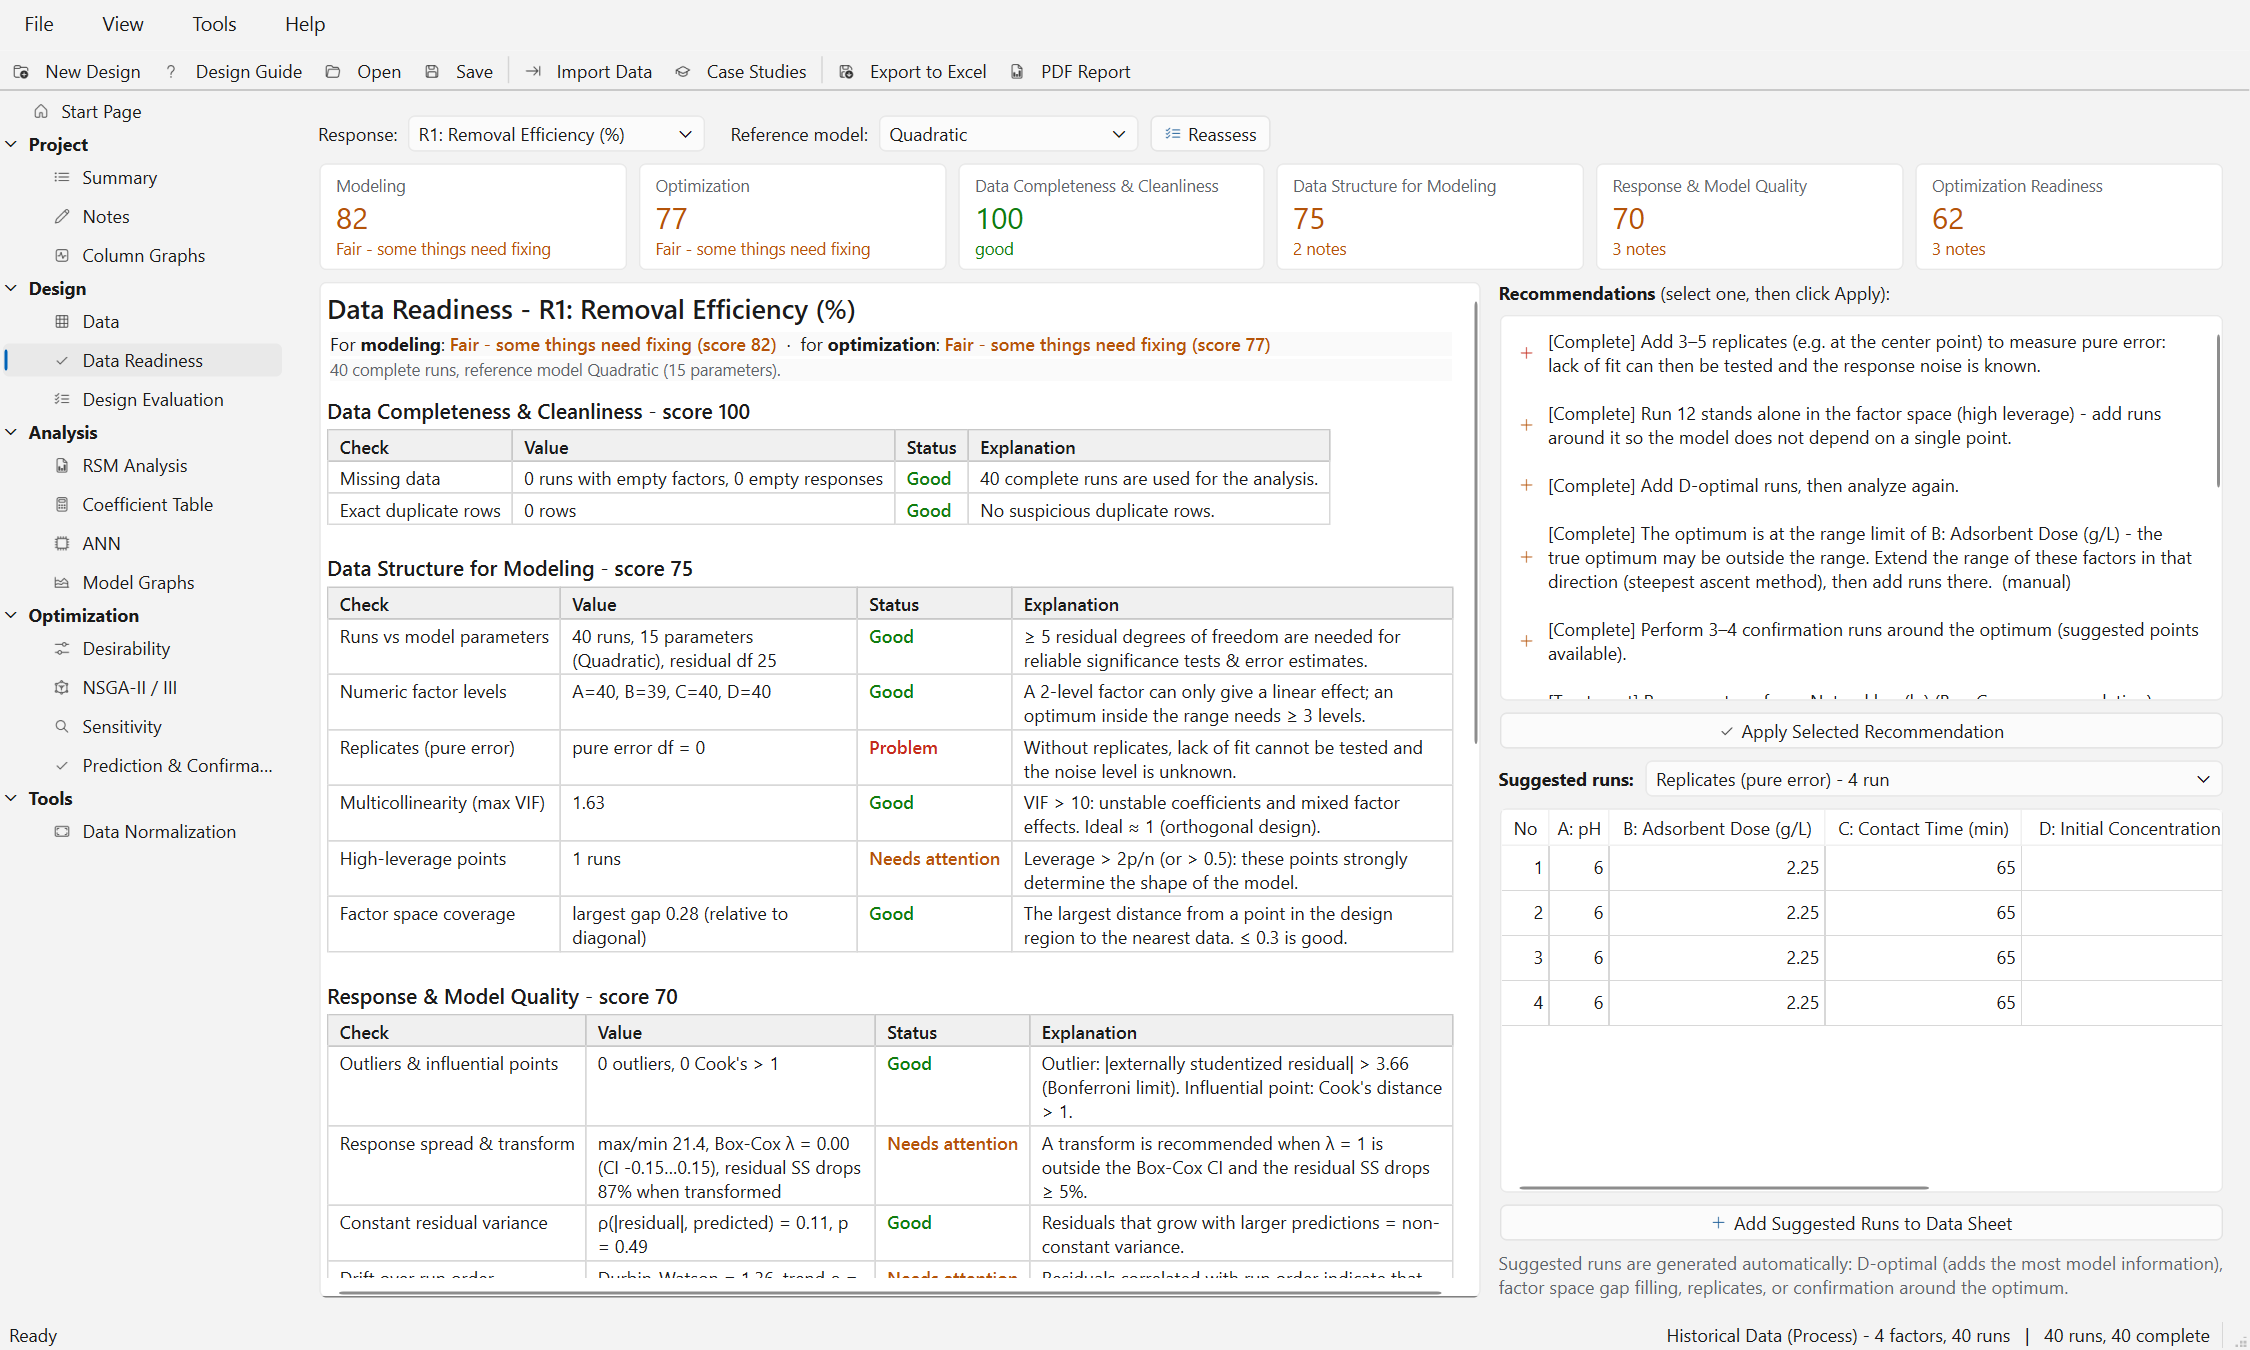
\includegraphics[width=\linewidth]{readiness_dye.png}
\caption{Data Readiness of the dye adsorption case (40 historical runs): Modeling 82 and Optimization 77, ``Fair -
some things need fixing''; the suggested runs show four replicates at the center.}
\label{fig:ch04-readinessdye}
\end{figure}

\paragraph{An unreplicated screening factorial.} For the 2\textsuperscript{4} fermentation case (Biomass, 2FI
model) the scores are 89 and 85. The structure checks flag 2 levels per factor (Needs attention, because the 2FI
model has no squared terms), pure-error df 0 (Problem) and a coverage gap of 0.48 (the interior of the cube holds no
runs). These are the expected limits of a screening design, not errors; the suggested middle-level runs, center
replicates and gap-filling runs are exactly the next stage of a sequential experiment (compare the augmentation to a
CCD in Chapter~\ref{chap:3}).

\paragraph{Limitations.} The assessment refers to one response and one reference model at a time; for GLM
(binomial, Poisson) and split-plot (REML) responses only part of the checks apply. For split-plot responses the
checks ``Model fit'' and ``Model significance'' are Info checks (not counted in the scores): R², adjusted and
predicted R² and an overall model F test are not defined for the REML model, which is judged by the Wald F tests of
its terms on the \ui{Split-Plot (REML)} tab of the RSM Analysis page (Chapter~\ref{chap:5}). Passing all checks does not prove that a model is right:
confirmation runs remain the final test.

\section{Design Evaluation}
\label{sec:ch04-eval}

\paragraph{Purpose.} \ui{Design Evaluation} judges the design matrix itself: how many degrees of freedom are left,
which terms are aliased, how precisely each coefficient can be estimated, how likely an effect of a given size is to
be detected (power), how correlated the model terms are and how the prediction variance is distributed over the
region. No response data are needed, so the page can be used before the experiment, to compare candidate designs, or
afterwards to assess historical data.

\paragraph{How to use.} Open \ui{Design Evaluation} in the group \ui{Design}, select the \ui{Model to evaluate:},
enter the effect size to detect (\ui{Signal $\Delta$:}) and the expected noise (\ui{Noise $\sigma$:}), choose
\ui{$\alpha$:} and the \ui{Graph:}. All runs with complete factor values are used, except excluded runs; blocks are
included in the model when the design has more than one block.

\begin{table}[htbp]
\centering
\caption{Options of the Design Evaluation page.}
\label{tab:ch04-evalopts}
\small
\begin{tabularx}{\linewidth}{@{}p{3.2cm}p{5.2cm}p{2.0cm}X@{}}
\toprule
Option & Values & Default & Meaning \\
\midrule
\ui{Model to evaluate:} & model orders of the design & design default & model whose coefficients are judged \\
\ui{Signal $\Delta$:} & 0.01--10\textsuperscript{6} & 2 & response difference between low and high level to detect \\
\ui{Noise $\sigma$:} & 0.0001--10\textsuperscript{6} & 1 & standard deviation of the response noise \\
\ui{$\alpha$:} & 0.01, 0.05, 0.1 & 0.05 & significance level of the tests \\
\ui{Graph:} & Fraction of Design Space (FDS), Prediction Std. Error Contour, Leverage per Run, Coefficient
Correlation Matrix, Pearson r Between Terms & FDS & plot on the right \\
\bottomrule
\end{tabularx}
\end{table}

Only the ratio $\Delta/\sigma$ matters for the power; $\sigma$ also scales the standard errors in the plots. A
practical choice is $\sigma$ = the expected repeatability of the measurement and $\Delta$ = the smallest change of
the response that matters in practice.

\subsection{Report}
\begin{itemize}
\item \textbf{Degrees of Freedom}: number of runs $n$, model coefficients $p$ (including intercept and block
columns), residual $n - p$, lack of fit and pure error. Notes appear when there is no residual df, fewer than 3
pure-error df or fewer than 3 lack-of-fit df. The box recalls the recommendation: at least 3 lack-of-fit df, 4
pure-error df and 5 residual df.
\item \textbf{Terms that cannot be estimated (aliased)}: model columns that are linear combinations of earlier
columns (QR rank check with tolerance $10^{-8}\max(1, \max|X|)\max(n, p)$); they are dropped.
\item \textbf{Coefficients}: per term the standard error (in units of $\sigma$), VIF, $R_i^2$ and power (green when
$\ge 80\,\%$).
\item \textbf{Alias Structure}: for each model term, the higher-order terms that bias its estimate.
\item \textbf{Matrix Measures}: condition number, determinant and trace of $(X^\top X)^{-1}$, D-, A- and
G-efficiency, average prediction variance I and $n \cdot I$, maximum and minimum prediction variance, maximum and
mean leverage.
\item \textbf{Correlation Between Terms (Pearson r)}: up to 10 pairs with $|r| \ge 0.3$ (red when $|r| \ge 0.7$), or
the note that no pair reaches 0.3, and the maximum $|r|$.
\item \textbf{Leverage}: mean and maximum.
\end{itemize}

\subsection{Theory as implemented}
Let $X$ be the $n \times p$ model matrix in coded units: intercept (omitted for Scheff\'e mixture models), block
columns (sum-to-zero coding), model terms (categorical factors effect coded), aliased columns removed. Let
$C = (X^\top X)^{+}$.

\paragraph{Standard error, VIF and leverage.}
\begin{equation}
SE_j = \sqrt{C_{jj}} \ (\times\sigma), \qquad
\text{VIF}_j = C_{jj} \sum_{i} (x_{ij} - \bar x_j)^2, \qquad R_j^2 = 1 - \frac{1}{\text{VIF}_j}, \qquad
h_i = x_i^\top C\, x_i .
\label{eq:ch04-se}
\end{equation}
VIF = 1 means the term is orthogonal to all others; VIF $> 10$ indicates strong collinearity \citep{belsley1980}.
VIF is not computed for the intercept nor for mixture models without intercept (the Scheff\'e terms are correlated
by construction). The mean leverage is $p/n$; a leverage close to 1 means the run alone determines part of the
model.

\paragraph{Degrees of freedom.} Pure-error df $= n - $ the number of distinct points (same block, coordinates rounded
to 6 decimals); lack-of-fit df $= (n - p) - df_{PE}$.

\paragraph{Power.} Each non-intercept coefficient is tested with a two-sided $t$ test with $n - p$ df. An effect
$\Delta$ between the low ($-1$) and high ($+1$) level corresponds to a coefficient $\beta = \Delta/2$; the
noncentrality parameter and the power are \citep{montgomery2017}
\begin{equation}
\lambda_j = \frac{\Delta/2}{\sigma\, SE_j}, \qquad
\text{Power}_j = 1 - F_{t'}\bigl(t_c;\, n-p,\, \lambda_j\bigr) + F_{t'}\bigl(-t_c;\, n-p,\, \lambda_j\bigr),
\qquad t_c = t_{1-\alpha/2,\, n-p},
\label{eq:ch04-power}
\end{equation}
where $F_{t'}$ is the cumulative distribution of the noncentral $t$ distribution. For a squared term the same
$\beta = \Delta/2$ is used. For mixture terms the ``low to high'' interpretation does not apply directly; use the
power only to compare mixture designs with each other.

\paragraph{Alias matrix.} The potential terms are those of the next higher model order (linear $\rightarrow$ 2FI,
2FI $\rightarrow$ 3FI, quadratic and special cubic $\rightarrow$ cubic) that are not in the model. With $X_2$ their
columns,
\begin{equation}
A = (X^\top X)^{+} X^\top X_2, \qquad E(\hat\beta) = \beta + A\,\beta_2 ,
\label{eq:ch04-alias}
\end{equation}
and every entry $|A_{jl}| > 10^{-6}$ is listed \citep{myers2016}. No alias table is shown for combined
mixture--process models.

\paragraph{Prediction variance and FDS.} The variance of the predicted mean at a point $x$ is
$v(x) = f(x)^\top C\, f(x)$, in units of $\sigma^2$; its square root is the prediction standard error. The Fraction of
Design Space plot \citep{myers2016} draws 4000 random points of the region (uniform in the box, Dirichlet for
mixtures, constraints respected), sorts their standard errors and plots them against the fraction of the region;
dotted lines and labels mark the standard error at 50\,\% and 80\,\% of the region. A low, flat curve is good.

\paragraph{Matrix measures.} With 3000 random region points $\mathcal{R}$ for the average prediction variance:
\begin{align}
\text{D-efficiency} &= 100\,\frac{|X^\top X|^{1/p}}{n}, &
\text{A-efficiency} &= 100\,\frac{p}{n \operatorname{tr} C}, \label{eq:ch04-deff}\\
\text{G-efficiency} &= 100\,\frac{p_m}{n \max_{x \in \mathcal{G}} v(x)}, &
I &= \operatorname{mean}_{x \in \mathcal{R}} v(x), \quad n \cdot I . \label{eq:ch04-geff}
\end{align}
For the G-efficiency, $p_m$ counts the model columns only (block columns are left out of both $p_m$ and $v(x)$), and
the maximum is taken over the set $\mathcal{G}$ of the design points, the corners of the region (the vertices for
mixtures and for constrained process regions, crossed with all levels of the categorical factors) and the 3000
random points. Because the design points and the corners are included, the worst prediction variance is not missed
and the G-efficiency does not exceed 100\,\% (for example, a 2\textsuperscript{7-4} design with its fold-over
gives 100\,\%). The page describes it as ``worst prediction variance in the design region (design points, corners or
vertices, random points); block terms excluded''. The condition number is $\lambda_{\max}/\lambda_{\min}$ of $X^\top X$ (1 = orthogonal, $> 100$ multicollinear,
$> 1000$ severe). The efficiencies are relative to an ideal orthogonal design with coded levels $\pm 1$ and are
computed in coded units; they are meant for comparing designs, also with different numbers of runs, or for assessing
historical data. Three limitations should be kept in mind: (1) for mixtures the pseudo-components range from 0 to 1,
so the efficiencies are much lower by construction and are only comparable between mixture designs; (2) with more
than 12 process factors no corners are used, and when the corners crossed with the categorical levels exceed 4096
combinations a random subset of 4096 is used, so the maximum of $v(x)$ can then be slightly underestimated; (3) for a
design with points outside the $\pm 1$ cube (a rotatable CCD) the average $I$ and the corners refer to the cube,
while the axial design points enter only the maximum of the G-efficiency.

\paragraph{Graphs.} \ui{Prediction Std. Error Contour}: contours of the prediction standard error over the first two
numeric factors (or a ternary plot of the first three components), other numeric factors at 0 (mixtures: the mean of
the design), categorical factors at their first level, with the design points; messages ``At least 2 numeric
factors (or 3 components) are required.'' and ``The slice is empty.''. \ui{Leverage per Run}: leverage in run order
with the reference line $2p/n$. \ui{Coefficient Correlation Matrix}: $C_{ab}/\sqrt{C_{aa}C_{bb}}$, the correlation
between the coefficient estimates. \ui{Pearson r Between Terms}: correlation between the model columns. Both heat
maps print the values when there are at most 16 terms.

\paragraph{Data export.} Every plot has \ui{Copy data} and \ui{Export data\dots} in its toolbar and right-click menu
(the FDS curve, the contour grid, the leverages or the matrices); the report has \ui{Export all tables\dots} in its
right-click menu.

\subsection{Examples}
\paragraph{BBD extraction case.} With the quadratic model, $\Delta = 2$, $\sigma = 1$, $\alpha = 0.05$
(Figure~\ref{fig:ch04-eval}): 17 runs, 10 coefficients, 7 residual df, 3 lack-of-fit df and 4 pure-error df (from
the 5 center points). The standard errors are 0.3536 for A, B, C, 0.5 for the interactions and 0.4873 for the
squares; the VIFs are 1 and 1.006. The power is 68.1\,\% for the main effects, 40.8\,\% for the interactions and
42.5\,\% for the squared terms, all below 80\,\%: an effect of two noise standard deviations would often be missed.
Raising the signal to $\Delta = 3$ raises all powers; in practice, replicates or a larger design would be needed for
small effects. The alias table shows that A is biased by $+0.5\,\text{AB}^2 + 0.5\,\text{AC}^2 + 1\,\text{A}^3$ if
cubic terms are active. Matrix measures: condition number 11.53, D-efficiency 34.0\,\%, A-efficiency 28.9\,\%,
G-efficiency 43.2\,\% (the largest prediction variance, $1.36\sigma^2$, is at the corners of the cube, where a BBD
has no runs), I = 0.340, maximum leverage 0.75, mean 0.588. The FDS curve gives a standard error of
$0.548\sigma$ at 50\,\% and $0.668\sigma$ at 80\,\% of the region.

\begin{figure}[htbp]
\centering
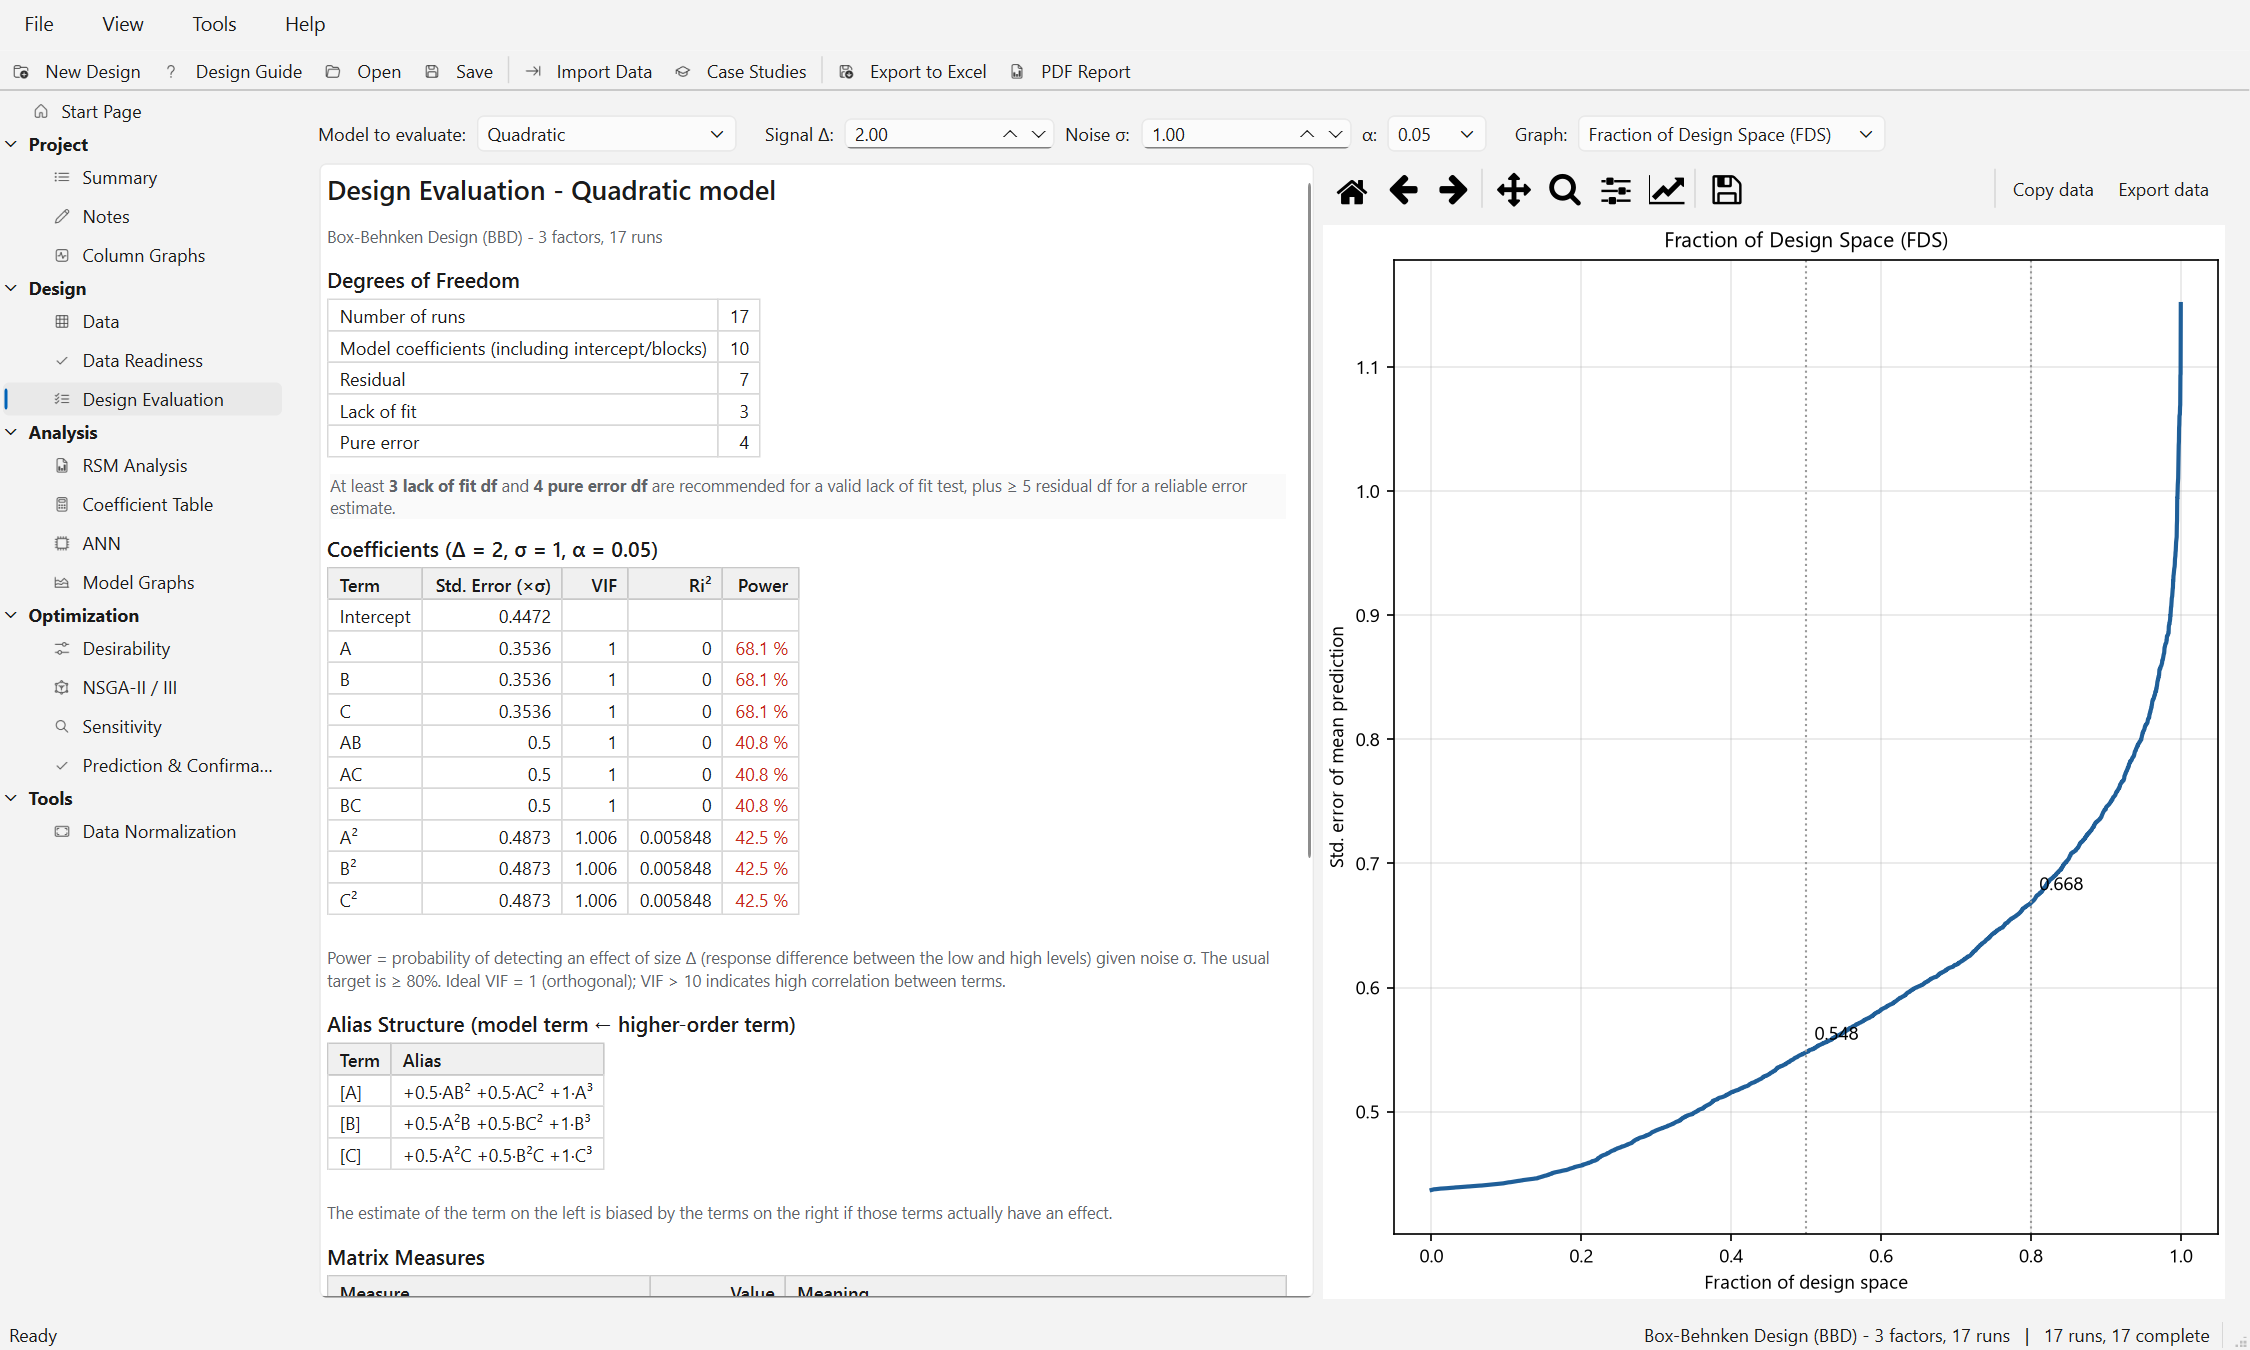
\includegraphics[width=\linewidth]{design_evaluation.png}
\caption{Design Evaluation of the BBD extraction case, quadratic model, $\Delta$ = 2, $\sigma$ = 1, $\alpha$ =
0.05: degrees of freedom, coefficients with standard error, VIF and power (red below 80 \%), alias structure, and the
FDS curve with the standard error at 50 \% (0.548) and 80 \% (0.668) of the region.}
\label{fig:ch04-eval}
\end{figure}

\paragraph{Comparing designs for three factors.} Table~\ref{tab:ch04-compare} compares five designs for the
quadratic model in three factors, computed on this page (seed 12345 for the optimal designs). The rotatable CCD has
the highest power and the lowest prediction variance, at the price of five levels and axial points outside the
range; the face-centered CCD estimates the squared terms poorly (power 32\,\%); the BBD saves three runs but has the
weakest interactions. The optimal designs estimate main effects and interactions very well but the squared terms
poorly, because with only $p = 10$ model points most points go to the boundary; their lack-of-fit and replicate
points are chosen for model checking, not for precision.

\begin{table}[htbp]
\centering
\caption{Design Evaluation of five three-factor designs, quadratic model, $\Delta = 2$, $\sigma = 1$, $\alpha =
0.05$.}
\label{tab:ch04-compare}
\footnotesize
\setlength{\tabcolsep}{4pt}
\begin{tabular}{@{}lccccc@{}}
\toprule
& CCD rotatable & CCD face & BBD & I-optimal & D-optimal \\
\midrule
Runs (residual / pure-error df) & 20 (10 / 5) & 20 (10 / 5) & 17 (7 / 4) & 20 (10 / 5) & 20 (10 / 5) \\
Power main effects (\%) & 91.4 & 81.3 & 68.1 & 94.0--95.2 & 93.7--93.9 \\
Power interactions (\%) & 72.2 & 72.2 & 40.8 & 90.3--92.9 & 87.3--90.2 \\
Power squared terms (\%) & 92.7 & 32.3 & 42.5 & 28.1--34.3 & 22.6--32.7 \\
Condition number & 12.9 & 20.3 & 11.5 & 58.7 & 53.1 \\
D-efficiency (\%) & 61.6 & 36.7 & 34.0 & 45.9 & 44.3 \\
A-efficiency (\%) & 51.6 & 26.5 & 28.9 & 22.3 & 20.9 \\
G-efficiency (\%) & 74.7 & 63.0 & 43.2 & 75.3 & 58.1 \\
I (average prediction variance) & 0.213 & 0.294 & 0.340 & 0.457 & 0.448 \\
$n \cdot I$ & 4.26 & 5.89 & 5.78 & 9.14 & 8.96 \\
FDS SE at 50\,\% / 80\,\% & 0.438 / 0.504 & 0.531 / 0.647 & 0.548 / 0.668 & 0.680 / 0.728 & 0.663 / 0.719 \\
\bottomrule
\end{tabular}
\end{table}

\paragraph{A mixture design.} For the edible film case (14 runs, quadratic Scheff\'e model) the page reports 8
residual df, 4 pure-error df and 4 lack-of-fit df, which satisfies the recommendation. The D-efficiency of 3.2\,\%
is not a sign of a bad design: it reflects the 0--1 range of pseudo-components (limitation 1 above).

\section{Summary}
\label{sec:ch04-summary}

\paragraph{Purpose.} The \ui{Summary} page (title ``Project Summary'') gives an overview of the whole project on one
page, for checking and for reports.

\paragraph{Content.} The box at the top shows the design description, the number of runs and how many have complete
factors (and how many are excluded), the blocks, the number of whole plots, the mixture total and, for designs created in the New
Design dialog, the random seed; constraints follow. The table \emph{Factors} lists for each factor the type (Numeric, Component,
Categoric), the low and high limits, the minimum, maximum, mean and standard deviation of the data, the number of
unique levels and the POE $\sigma$ entered in Factor \& Response Info; categorical factors list their levels with
counts. The table \emph{Responses} lists the type (normal, binomial, poisson), the number of values used ($n$, without
excluded runs), minimum, maximum, mean, SD, the ratio max/min (relevant for a transform), the model (``(selected
terms)'' when terms were edited), the transform, R\textsuperscript{2} (McFadden R\textsuperscript{2} for GLM,
conditional R\textsuperscript{2} for split-plot), adjusted and predicted R\textsuperscript{2}, and the model used for
optimization (RSM or ANN with its architecture). A line ``Other project contents'' counts the ANN models, the
desirability solutions and the NSGA Pareto solutions; the notes close the page. The report panel supports
\ui{Export all tables\dots}.

\begin{figure}[htbp]
\centering
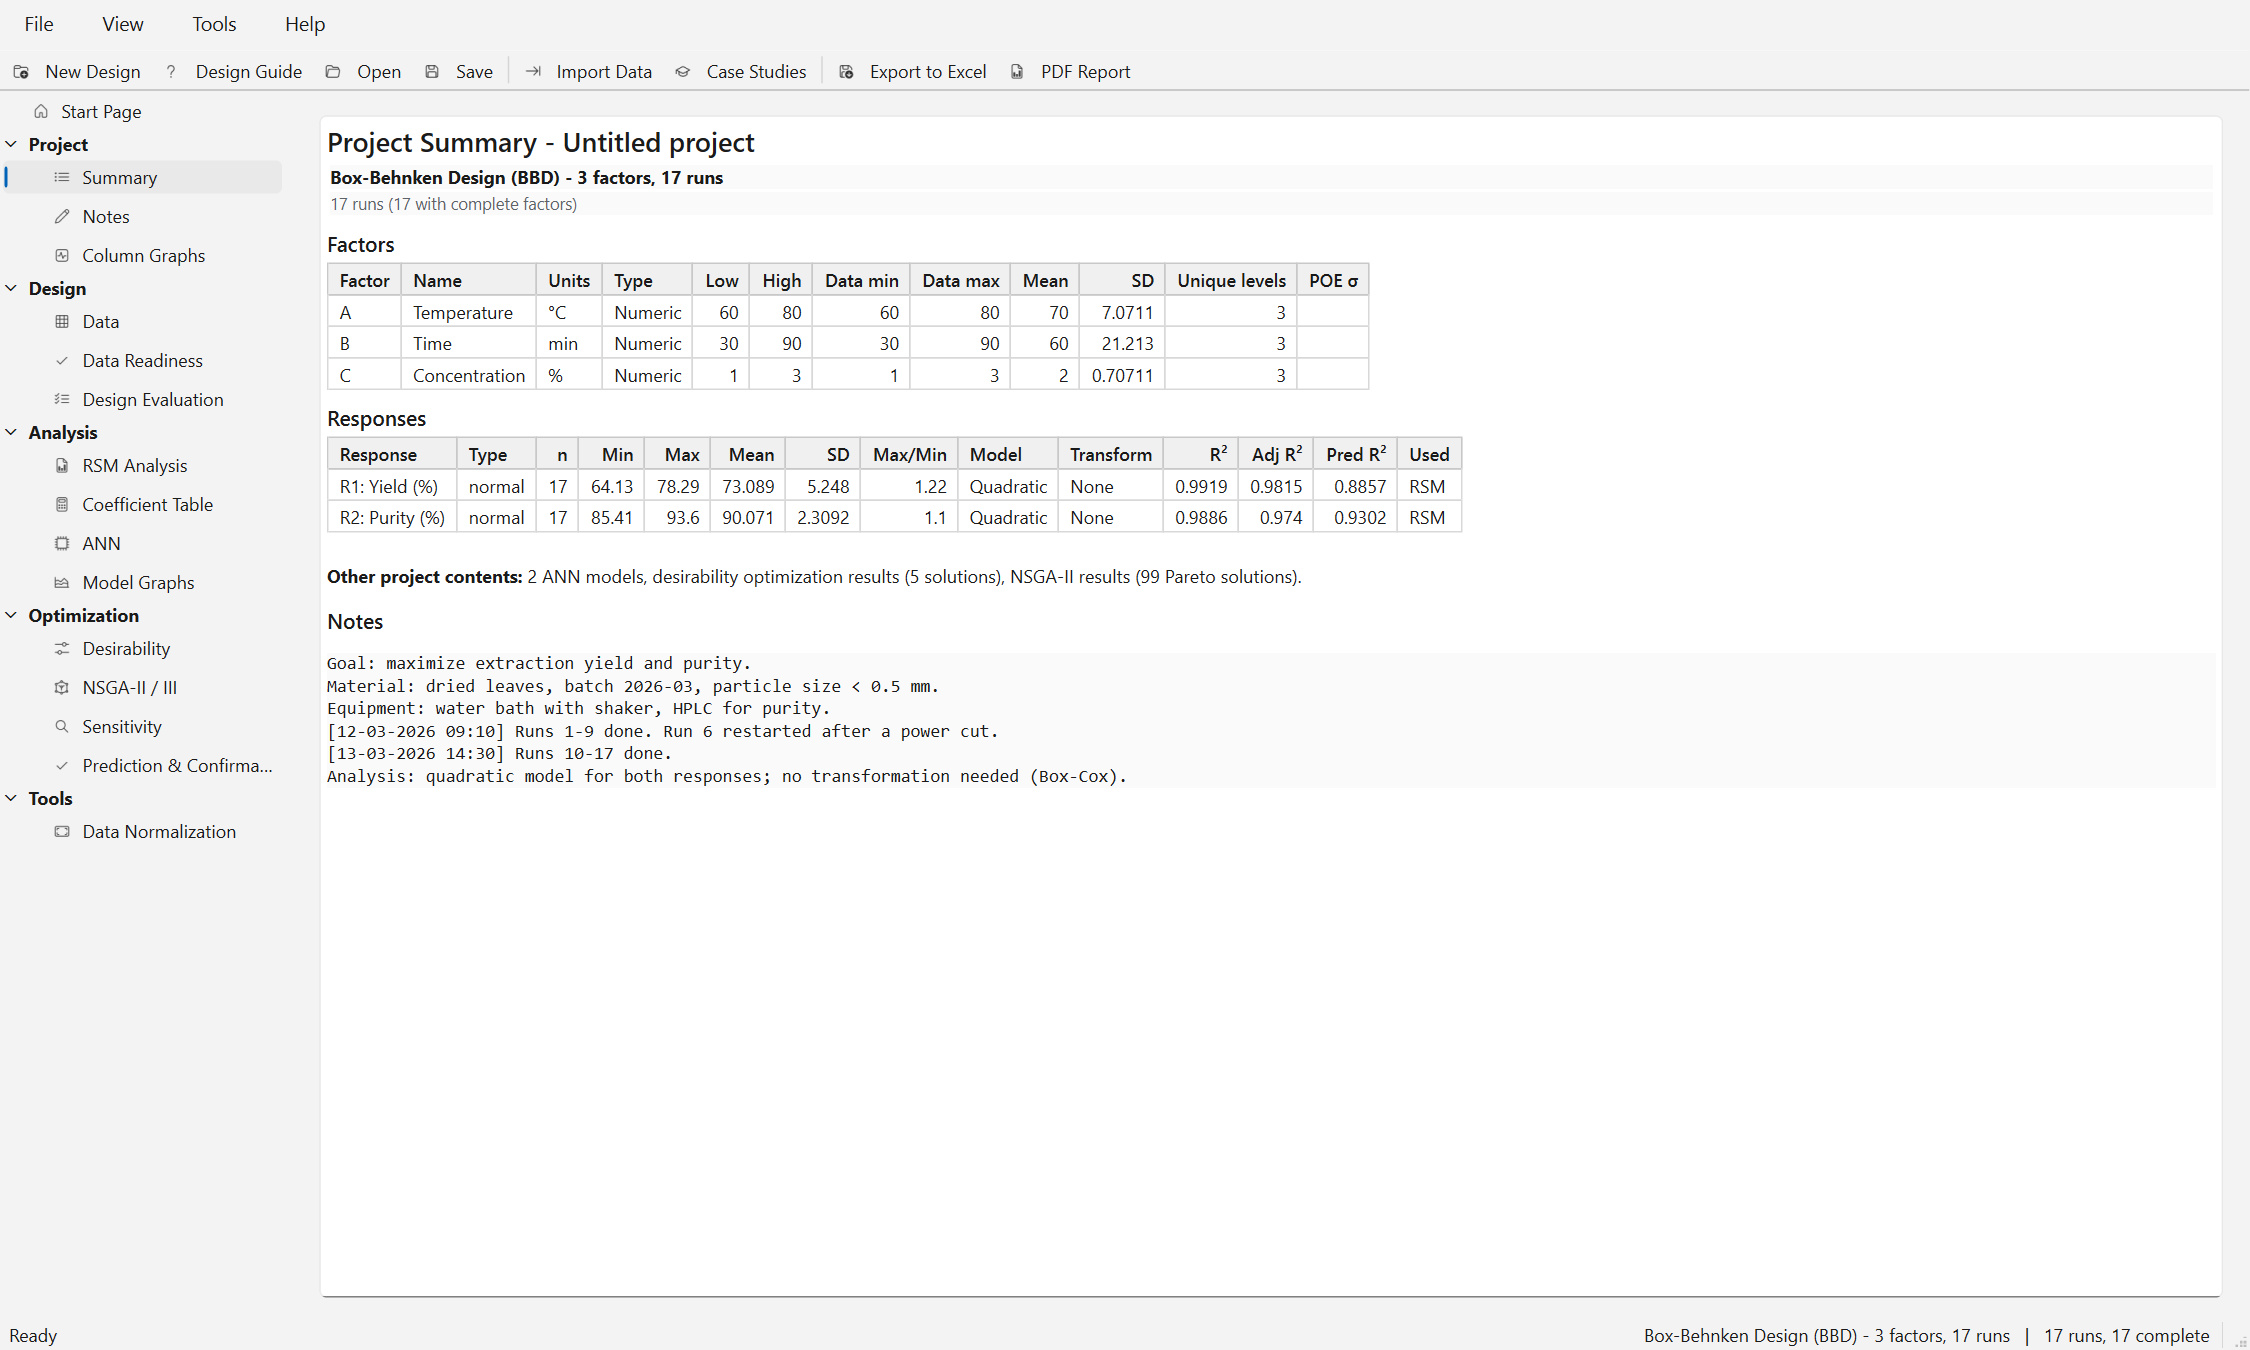
\includegraphics[width=\linewidth]{summary.png}
\caption{Summary of the BBD extraction case after the analysis: factor and response tables (Yield: quadratic,
R\textsuperscript{2} 0.9919, Adj R\textsuperscript{2} 0.9815, Pred R\textsuperscript{2} 0.8857; Purity:
R\textsuperscript{2} 0.9886, Adj 0.974, Pred 0.9302), 2 ANN models, 5 desirability solutions and 99 Pareto
solutions.}
\label{fig:ch04-summary}
\end{figure}

\section{Notes}
\label{sec:ch04-notes}
The \ui{Notes} page is a free text field for the experiment goals, equipment and material conditions, events during
the experiment and analysis decisions. \ui{Insert Date} inserts a time stamp ``[dd-mm-yyyy hh:mm]'' at the cursor.
The notes are saved in the \texttt{.doe} file, shown on the Summary page and printed in the PDF report. Good notes
make an experiment traceable: record deviations from the run order, failed runs and the reasons for excluding any
run.

\begin{figure}[htbp]
\centering
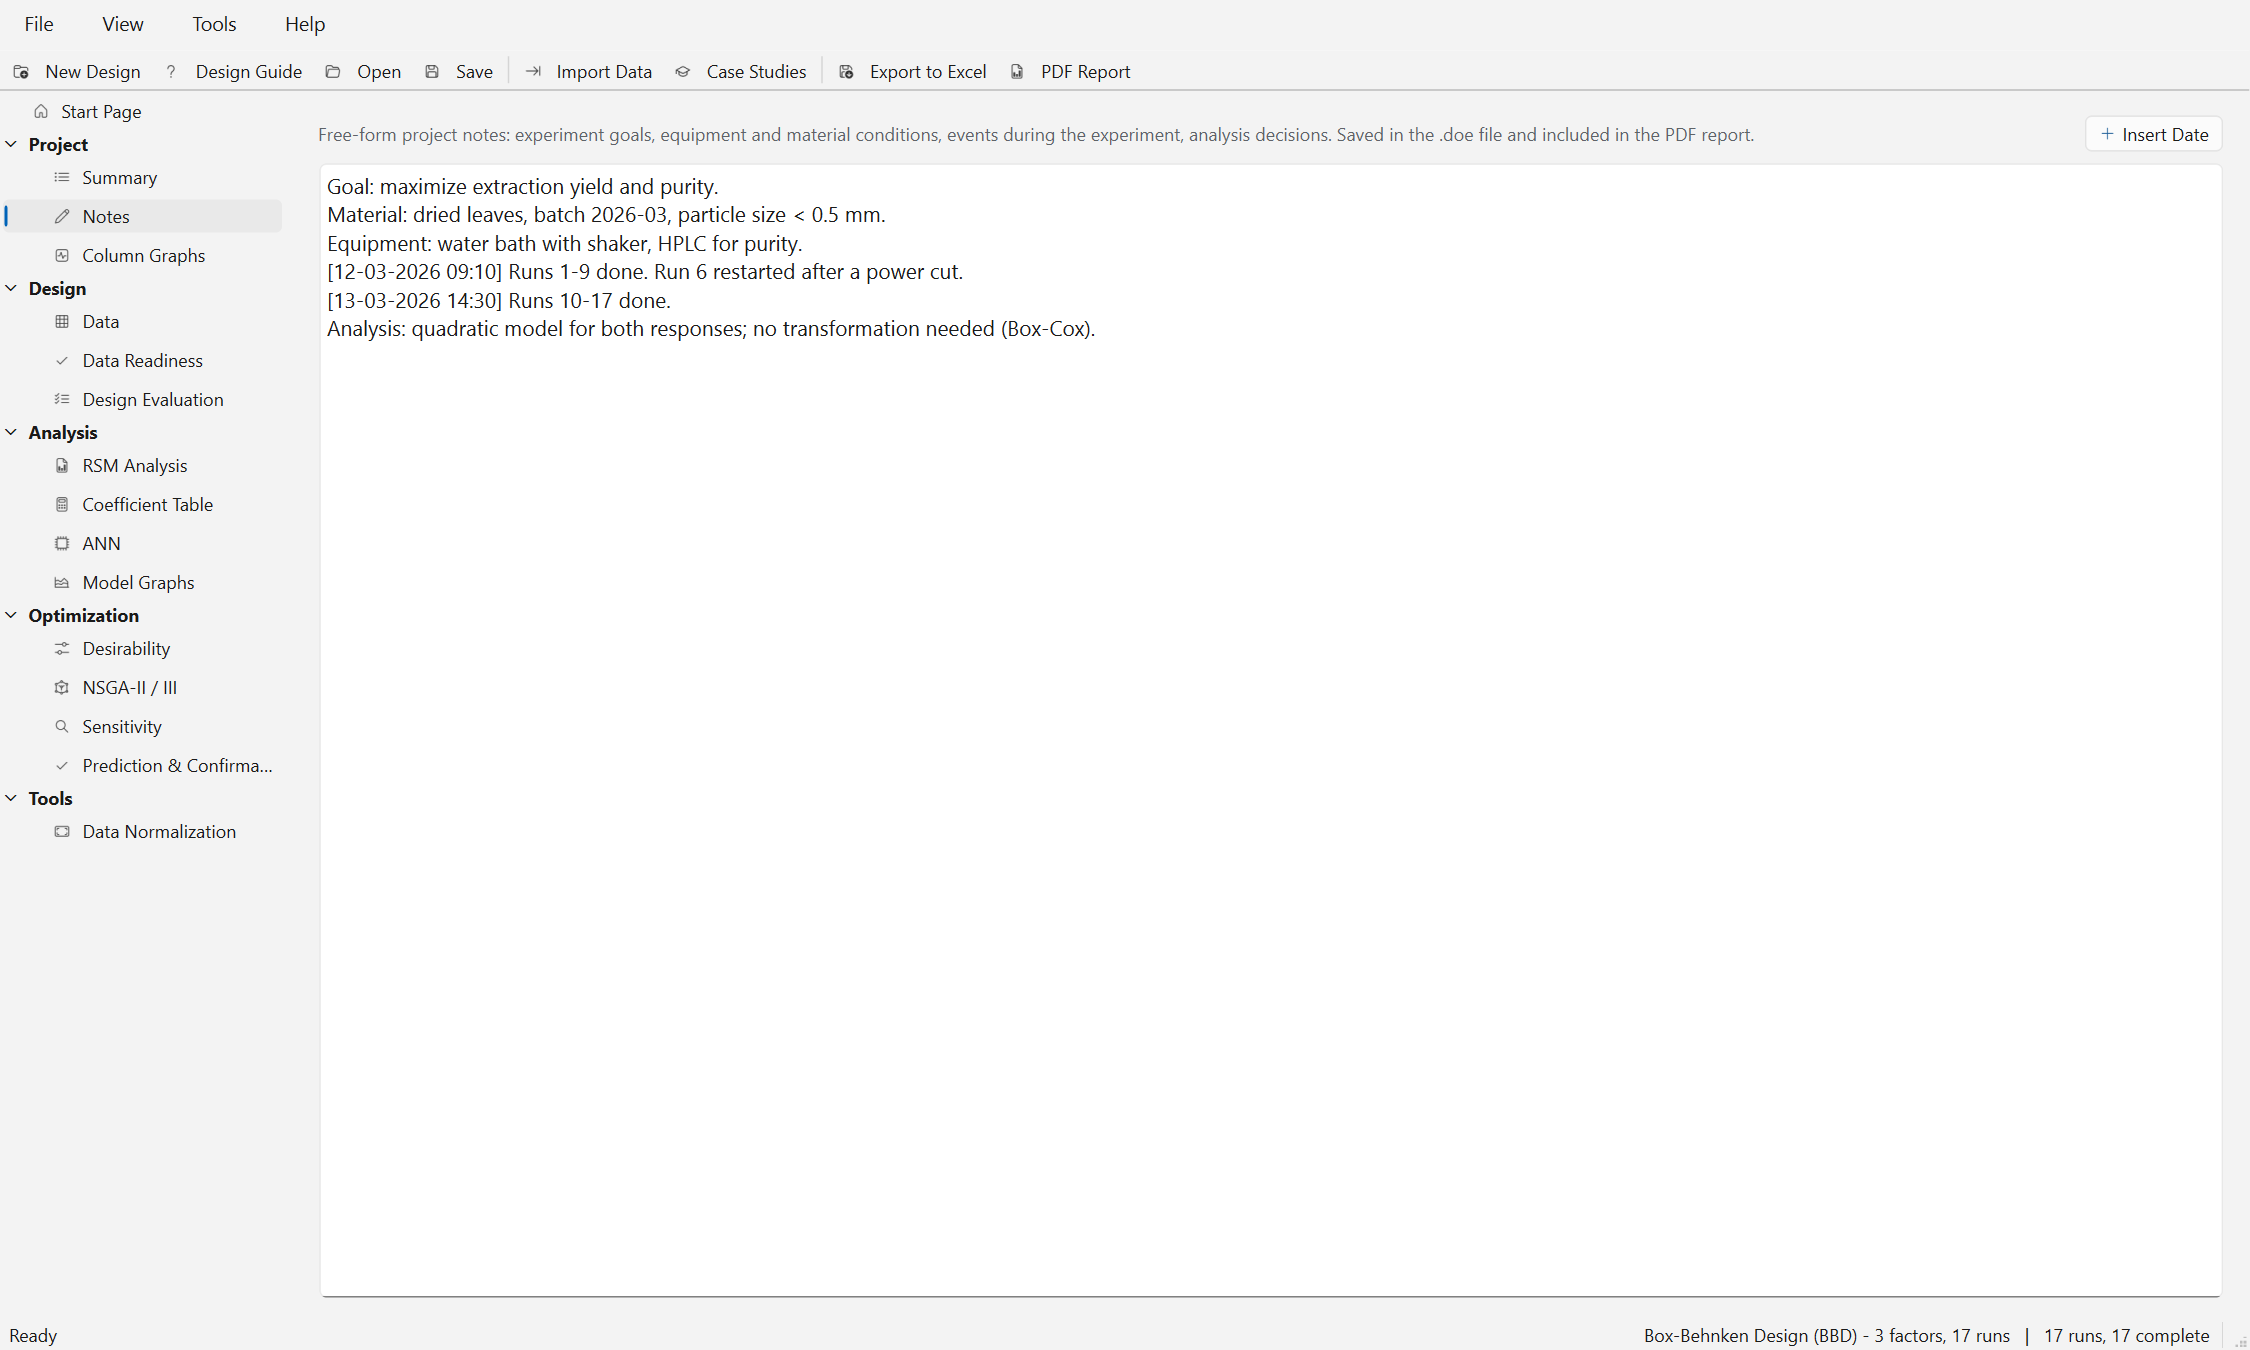
\includegraphics[width=0.85\linewidth]{notes.png}
\caption{Notes page with an example of goals, materials, equipment, dated events and an analysis decision.}
\label{fig:ch04-notes}
\end{figure}

\section{Column Graphs}
\label{sec:ch04-columns}

\paragraph{Purpose.} \ui{Column Graphs} explores the raw data columns before (and besides) modeling: distributions,
relations between factors and responses, trends over the run order and correlations in historical data.

\paragraph{Columns.} ``Std Order'', ``Run'', ``Block'' (if blocked), every factor in actual units (categorical
factors as level index with the level names on the axis), every response (excluded runs empty) and ``Residual R1'',
\dots{} for every least-squares response with a fitted model ($y - \hat y$).

\paragraph{Options.} \ui{Type:} \ui{Scatterplot} (default), \ui{Histogram}, \ui{Box plot}, \ui{Scatter matrix};
\ui{Color by:} (None or any column, default Run); \ui{X axis:} (default the first factor); \ui{Y axis:} (default the
first response); \ui{Z axis (3D):} (None, or a column for a 3-D scatter); \ui{Trend line (linear regression)}.

\paragraph{Output.}
\begin{itemize}
\item \emph{Scatterplot}: Y against X with the label ``Correlation (Pearson r) = \dots{} $\cdot$ Spearman $\rho$ =
\dots{} $\cdot$ n = \dots'' and, optionally, the least-squares line $y = a x + b$. Numeric colouring uses a continuous
color map with a color bar, categorical colouring a legend.
\item \emph{Histogram}: $\min(50, \max(8, \lfloor\sqrt{n}\rfloor))$ bins (a bar chart of counts for categorical
columns), with $n$, mean, SD, median and skewness.
\item \emph{Box plot}: Y grouped by the distinct values of X if X is categorical or has at most 12 distinct values,
otherwise by 5 quantile groups; the Kruskal--Wallis test reports whether the groups differ ($\alpha = 0.05$).
\item \emph{Scatter matrix}: up to the first 8 factor and response columns, histograms on the diagonal and $r$ in
each panel (red when $|r| \ge 0.5$); at most 2000 random complete runs are drawn.
\end{itemize}
The heat map on the right shows the Pearson correlation of all pairs of columns; clicking a cell plots that pair.
Correlations use the pairwise complete rows and need more than two rows. In a designed experiment the factor columns
are nearly uncorrelated; strong correlations between factors in historical data warn that their effects cannot be
separated (check VIF on the Design Evaluation page). A trend of a response or a residual against \ui{Run} indicates
drift. Every plot has \ui{Copy data} and \ui{Export data\dots}.

\begin{figure}[htbp]
\centering
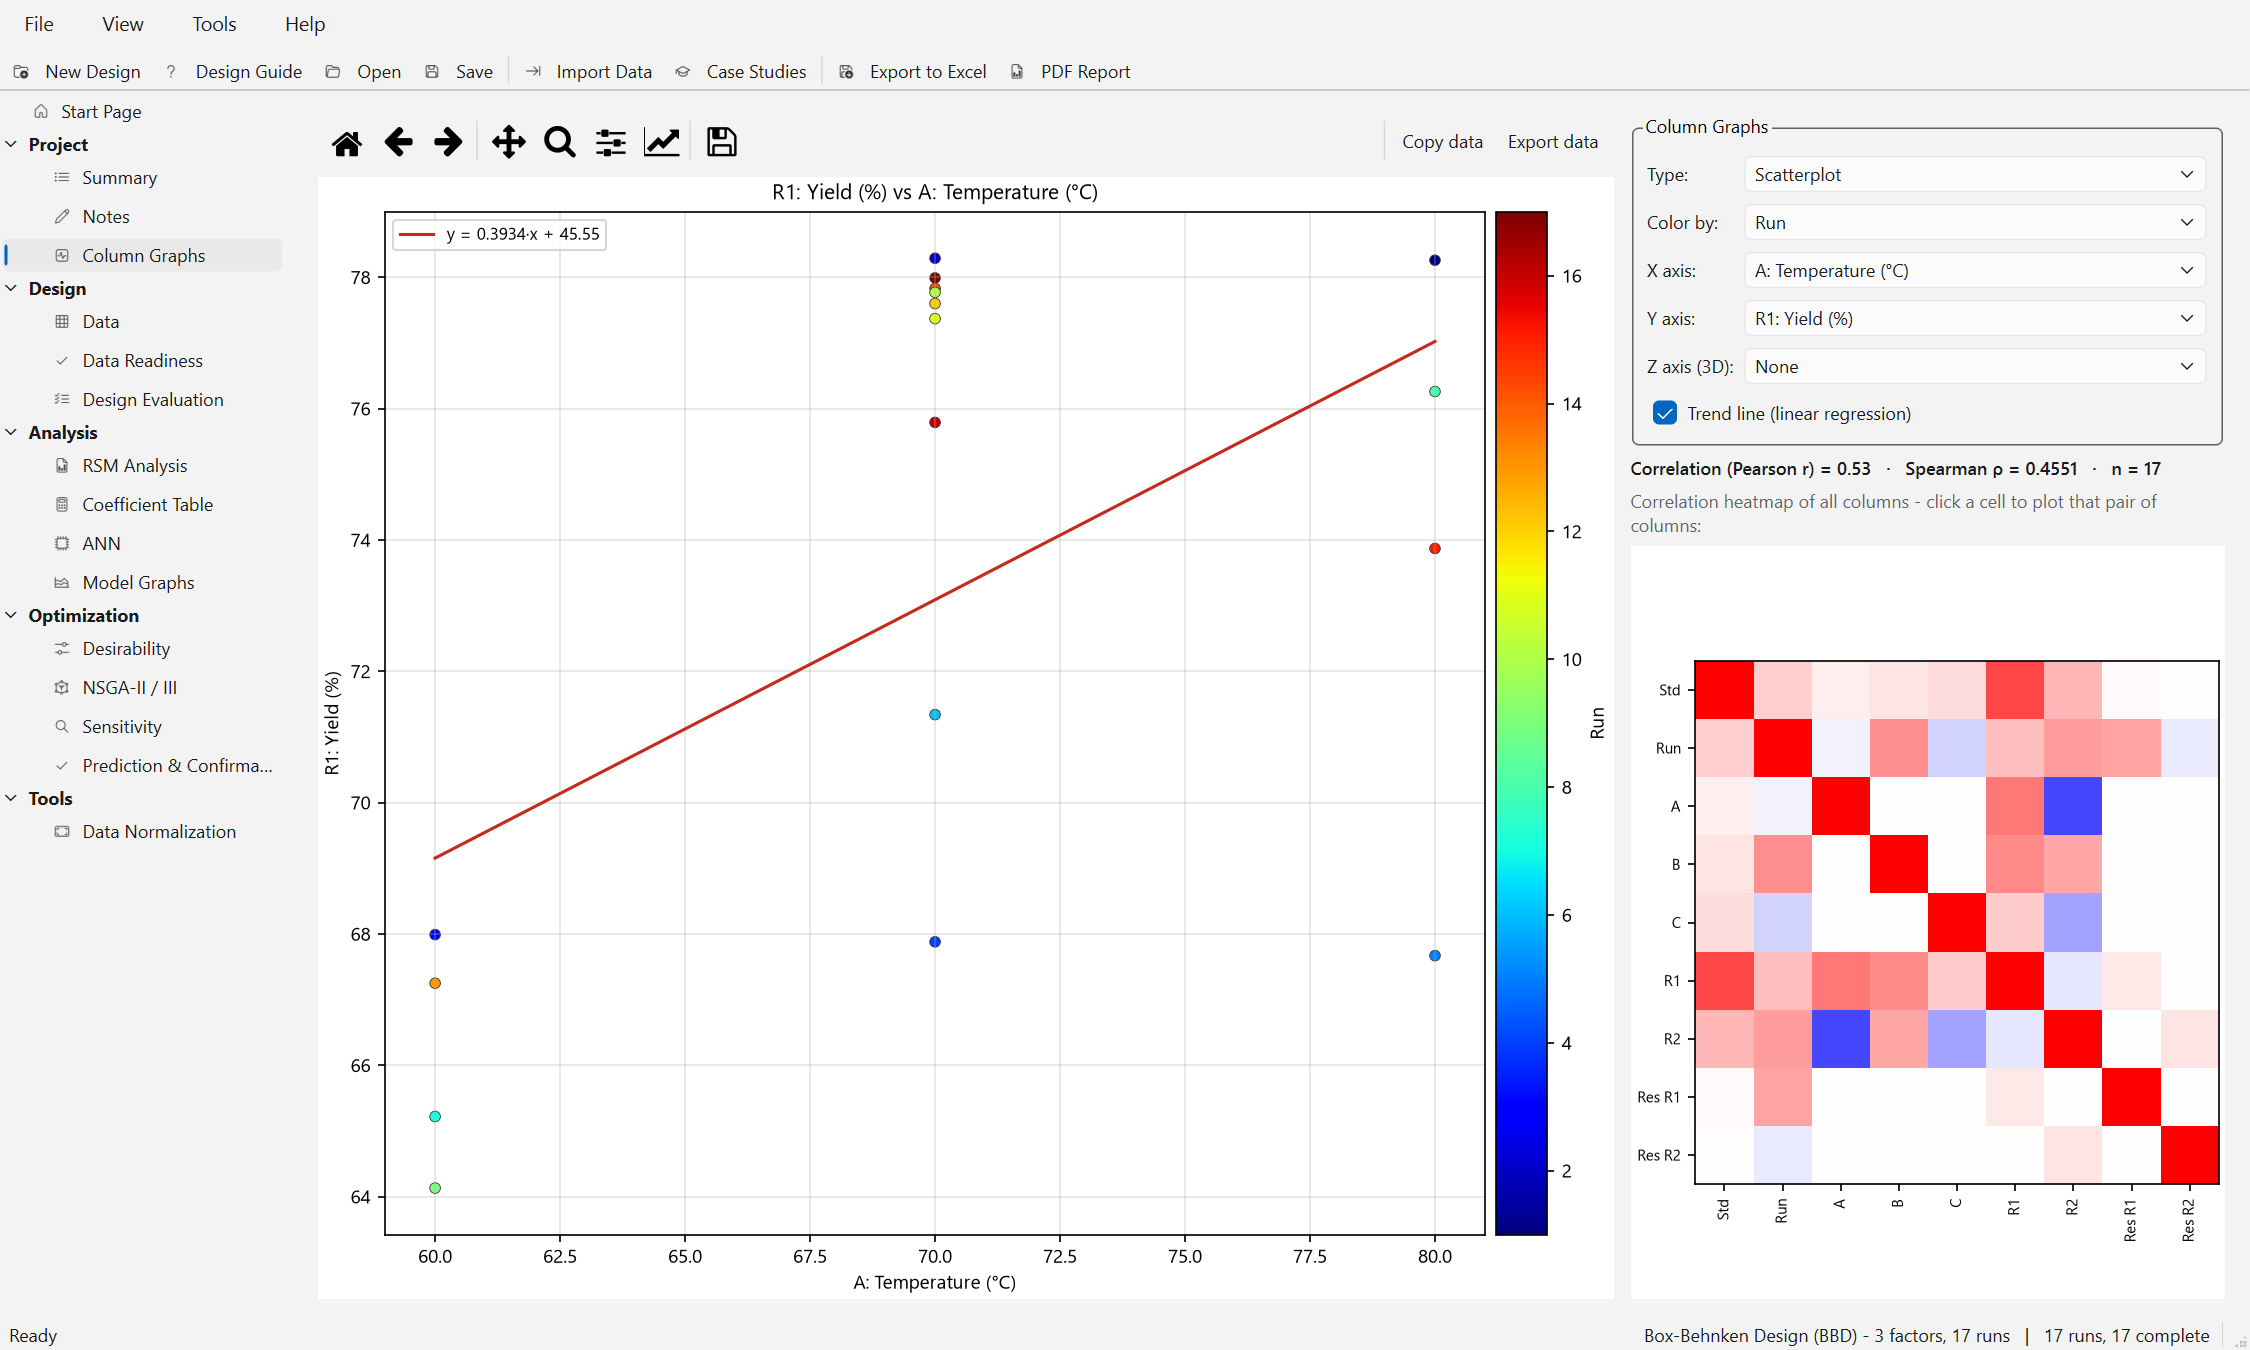
\includegraphics[width=\linewidth]{column_graphs.png}
\caption{Column Graphs for the BBD extraction case: Yield against Temperature, coloured by run, with the trend line
$y = 0.3934x + 45.55$, Pearson r = 0.53 and Spearman $\rho$ = 0.4551 ($n$ = 17); correlation heat map of all
columns.}
\label{fig:ch04-columngraphs}
\end{figure}

\paragraph{Example.} In Figure~\ref{fig:ch04-columngraphs} the linear correlation between Temperature and Yield is
only 0.53 although Temperature is the strongest factor: the effect is curved (a maximum inside the range), which a
correlation coefficient does not capture. This is why factor effects are judged from the model, not from raw
correlations.

\section{Coefficient Table}
\label{sec:ch04-coef}
The \ui{Coefficient Table} (group \ui{Analysis}) shows the coded coefficients of all responses side by side: one row
per model term, one column per response with a computable RSM model. A cell holds the coefficient (coded units or
pseudo-components) and, with \ui{Show p-values} on, its $p$-value; the background is dark green for $p < 0.01$, light
green for $p < 0.05$ and yellow for $p < 0.1$. An empty cell means that the term is not in that response's model.
The footer rows give the transform, the model, the model $p$-value, R\textsuperscript{2}, adjusted and predicted
R\textsuperscript{2} and the model used for optimization. Because the coefficients are in coded units, their sizes can
be compared across factors and responses: a factor with a large positive coefficient for one response and a large
negative one for another signals a trade-off that the optimization must resolve. For responses that use an ANN, the
table still shows the RSM coefficients. The $p$-values come from the same tests as in the RSM analysis; the theory is
given in Chapter~\ref{chap:5}. The report supports \ui{Export all tables\dots}.

\begin{figure}[htbp]
\centering
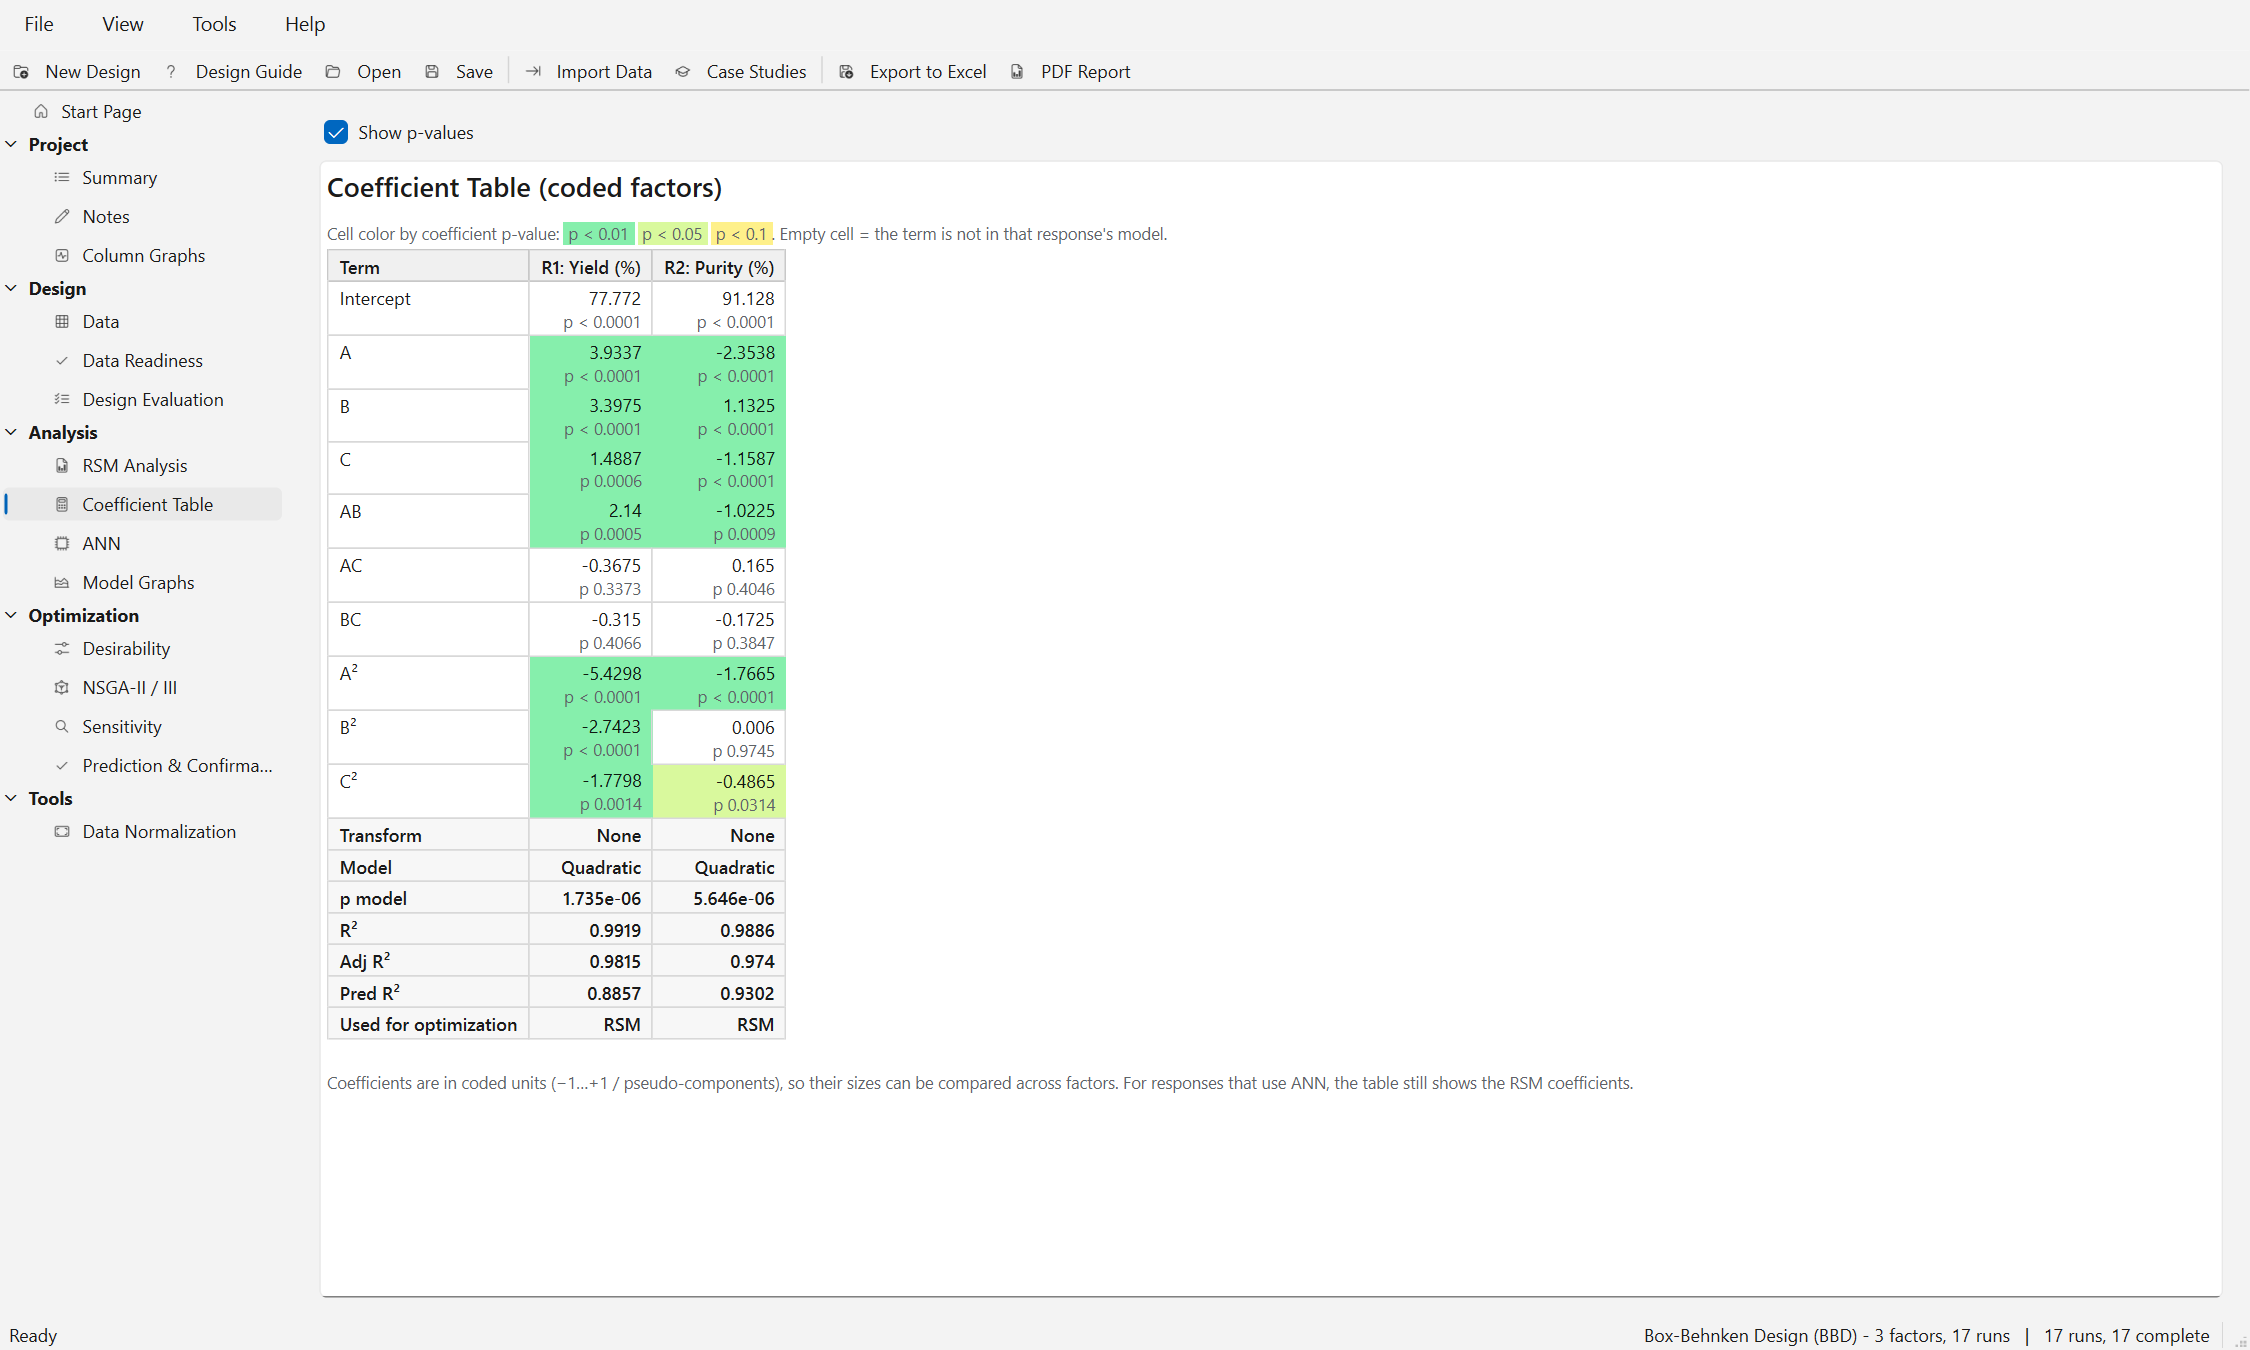
\includegraphics[width=\linewidth]{coefficient_table.png}
\caption{Coefficient Table of the BBD extraction case: Yield intercept 77.772, A 3.9337, A\textsuperscript{2}
$-5.4298$; Purity A $-2.3538$. AC and BC are not significant for either response.}
\label{fig:ch04-coef}
\end{figure}

\section{Data Normalization}
\label{sec:ch04-normalization}

\paragraph{Purpose.} Variables with different units and ranges (pH 2--10 and a concentration of 20--200 mg/L) are
put on a common scale so that no variable dominates only because its numbers are large. RSM uses coded factors
automatically, and the ANN normalizes its inputs and outputs with the method chosen on the ANN page; this page
(\menupath{Tools $\rightarrow$ Data Normalization}) is for viewing, comparing and exporting normalized data. It does
not change the project.

\paragraph{Options.} \ui{Method:} ``Min-max to [-1, 1] (mapminmax) - recommended'' (default), ``Min-max to [0,
1]'', ``Z-score standardization (mapstd): mean 0, SD 1'' and ``No normalization (for comparison)''; check boxes
\ui{Factors} and \ui{Responses} (both on); button \ui{Export to Excel\dots}.

\paragraph{Theory.} Every column is transformed as
\begin{equation}
x' = b + \frac{x - o}{s},
\label{eq:ch04-norm}
\end{equation}
with offset $o$, scale $s$ and base $b$:
\begin{center}
\small
\begin{tabular}{@{}lcccc@{}}
\toprule
Method & $o$ & $s$ & $b$ & Range of $x'$ \\
\midrule
mapminmax & $\min x$ & $(\max x - \min x)/2$ & $-1$ & $[-1, 1]$ \\
min-max [0, 1] & $\min x$ & $\max x - \min x$ & 0 & $[0, 1]$ \\
z-score (mapstd) & mean & SD ($n-1$) & 0 & mean 0, SD 1 \\
none & 0 & 1 & 0 & original \\
\bottomrule
\end{tabular}
\end{center}
A zero scale (a constant column) is replaced by 1; missing values are ignored. Categorical factors use the level
index. The data are all runs in run order, without the excluded runs (a note states how many are left out). The
minimum and maximum come from the data, not from the design limits, so a new value outside the observed range maps
outside $[-1, 1]$.

\paragraph{Output.} The tab \ui{Normalized Data} lists Run and the normalized columns (5 decimals); the tab
\ui{Statistics \& Parameters} lists for each variable the minimum, maximum, mean, SD, range, offset, scale, base and
the new minimum and maximum. The figure shows box plots before (original units) and after normalization (a random
sample of 5000 rows for very large data; factors and responses in different colors). \ui{Export to Excel\dots}
writes the sheets ``Normalized'' (method and formula in the first row), ``Original Data'' and ``Parameters'' (offset,
scale and base per variable, so the transformation can be reproduced). The tables support \ui{Export table\dots}
and the plot \ui{Copy data} and \ui{Export data\dots}.

\paragraph{Example.} In the dye adsorption case pH ranges from 2.13 to 9.97, so mapminmax uses $o = 2.13$ and
$s = 3.92$; Initial Concentration ranges from 22.1 to 198.6 ($s = 88.25$) and Removal Efficiency from 2.73 to 58.45
($s = 27.86$). The first run in run order (pH 4.93, dose 3.29 g/L, time 81.7 min, concentration 147 mg/L, removal
35.57 \%) becomes $(-0.286, 0.606, 0.305, 0.415, 0.179)$. Figure~\ref{fig:ch04-norm} shows how the very different
scales before normalization collapse into the common range.

\begin{figure}[htbp]
\centering
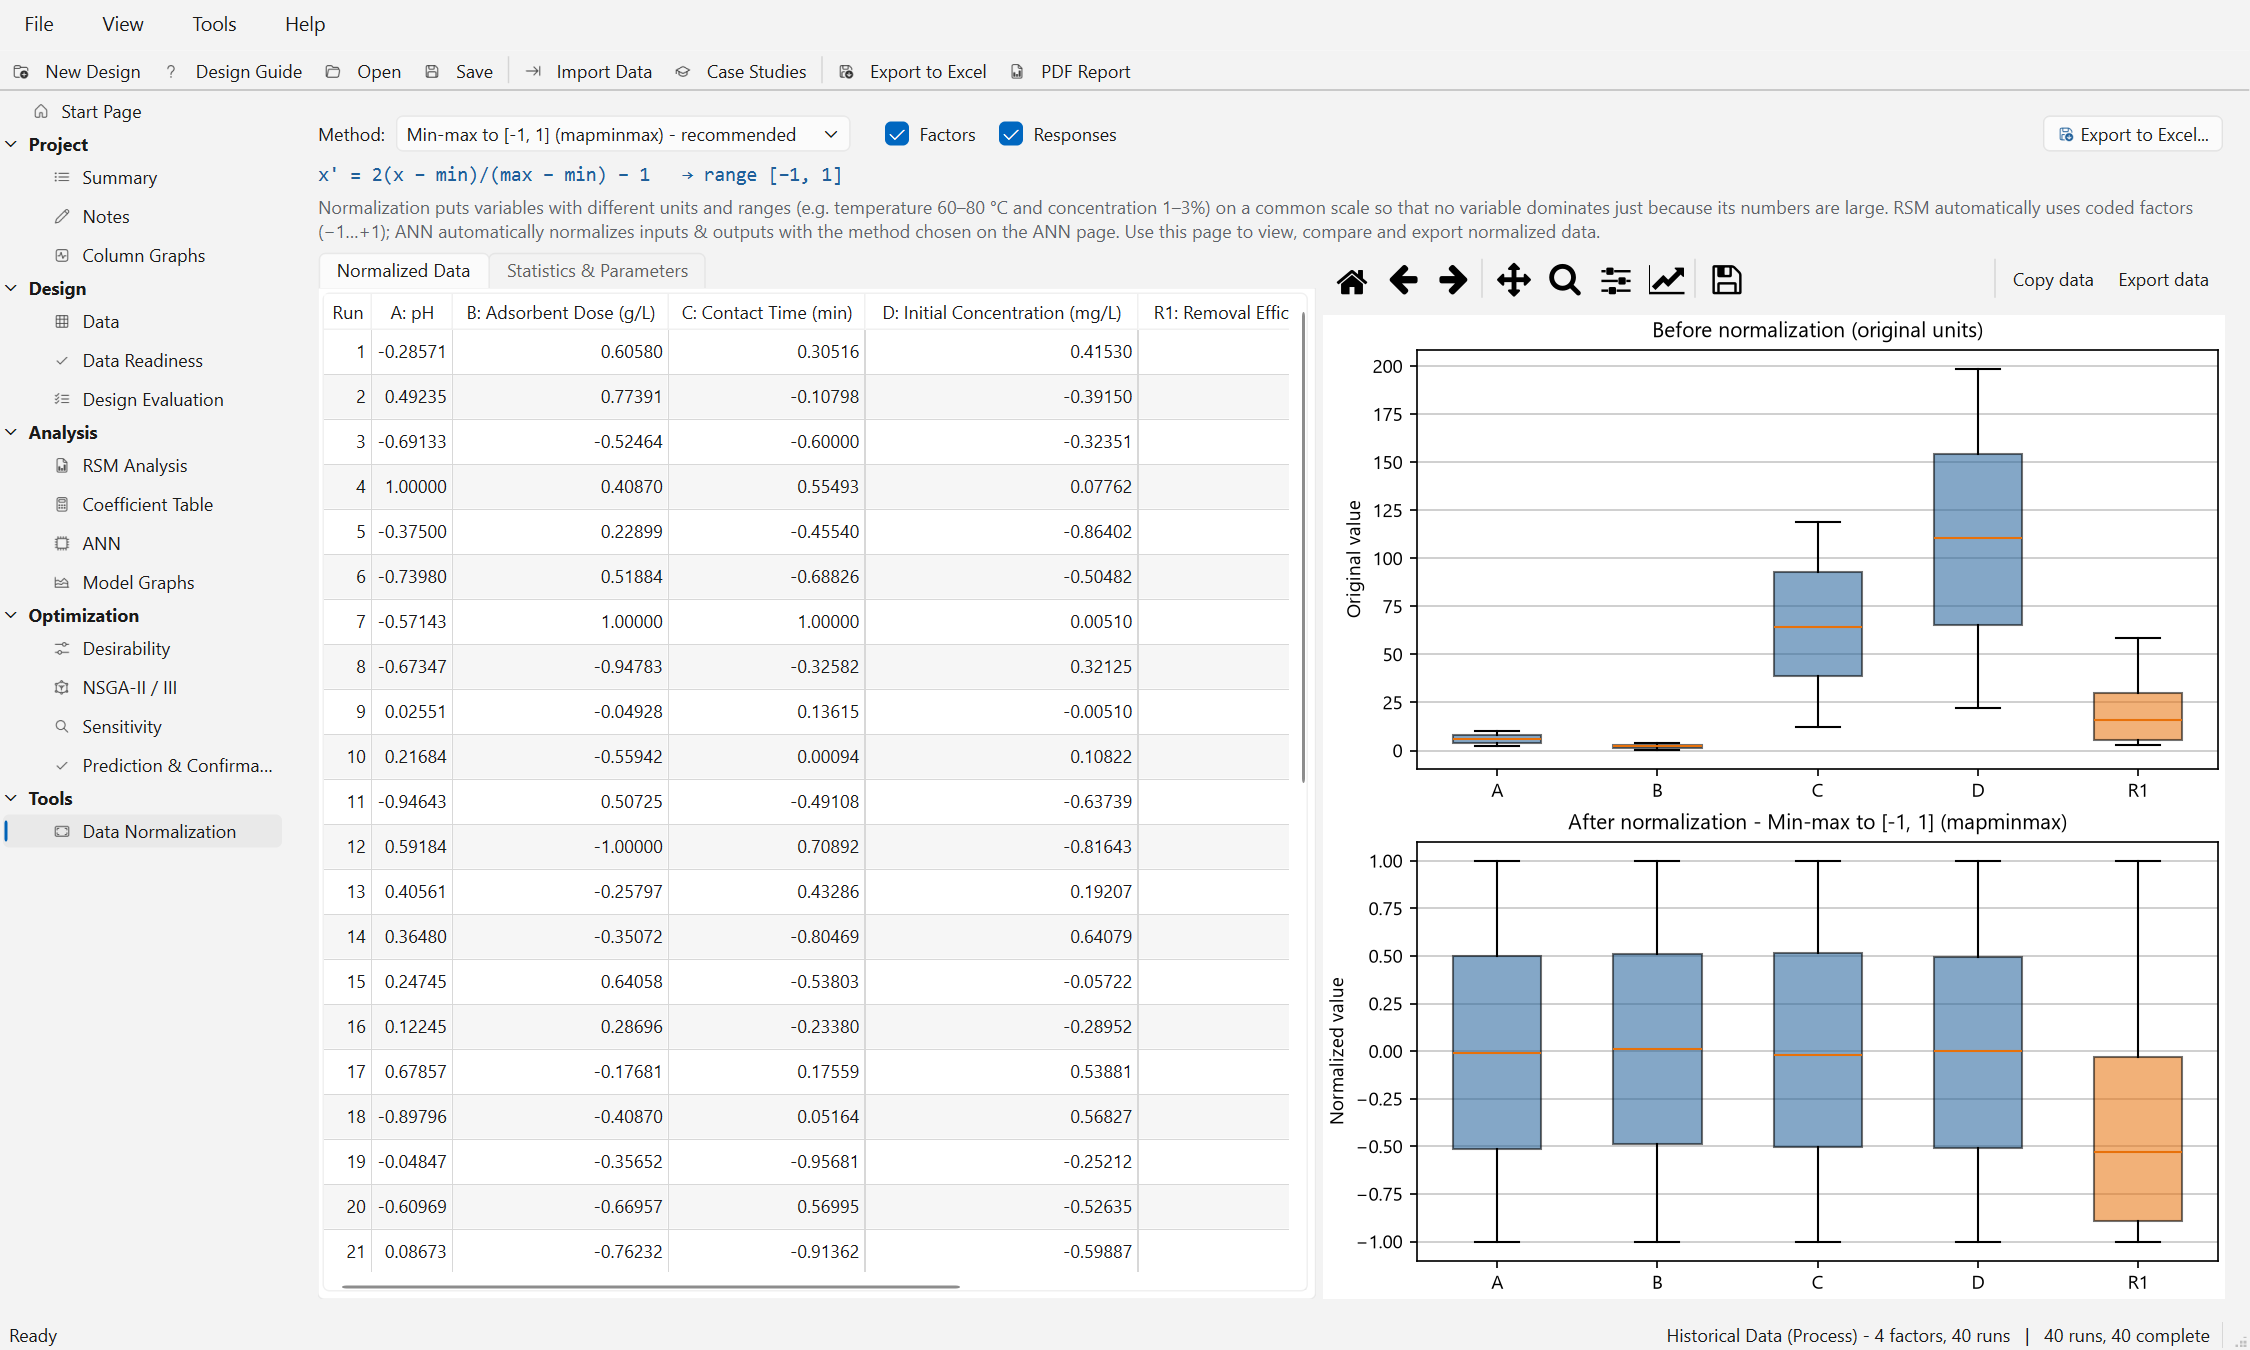
\includegraphics[width=\linewidth]{normalization.png}
\caption{Data Normalization of the dye adsorption case with mapminmax: formula, normalized data and box plots
before and after normalization.}
\label{fig:ch04-norm}
\end{figure}
